\documentclass[12pt letter]{report}
%%%%%%%%%%%%%%%%%%%%%%%%%%%%%%%%%
% PACKAGE IMPORTS
%%%%%%%%%%%%%%%%%%%%%%%%%%%%%%%%%


\usepackage[tmargin=2cm,rmargin=1in,lmargin=1in,margin=0.85in,bmargin=2cm,footskip=.2in]{geometry}
\usepackage{amsmath,amsfonts,amsthm,amssymb,mathtools}
\usepackage[varbb]{newpxmath}
\usepackage{xfrac}
\usepackage[makeroom]{cancel}
\usepackage{mathtools}
\usepackage{bookmark}
\usepackage{enumitem}
\usepackage{hyperref,theoremref}
\hypersetup{
  pdftitle={Assignment},
  colorlinks=true, linkcolor=doc!90,
  bookmarksnumbered=true,
  bookmarksopen=true
}
\usepackage[most,many,breakable]{tcolorbox}
\usepackage{xcolor}
\usepackage{varwidth}
\usepackage{varwidth}
\usepackage{etoolbox}
%\usepackage{authblk}
\usepackage{nameref}
\usepackage{multicol,array}
\usepackage{tikz-cd}
\usepackage[ruled,vlined,linesnumbered]{algorithm2e}
\usepackage{comment} % enables the use of multi-line comments (\ifx \fi) 
\usepackage{import}
\usepackage{xifthen}
\usepackage{pdfpages}
\usepackage{transparent}
\usepackage{xcolor,colortbl,array,amssymb}
\usepackage{venndiagram}
\usepackage{listings}
\usepackage{fontspec}

\setmainfont{LibertinusSerif}[
  Extension = .otf,
  Path = /usr/share/fonts/libertinus/,
  UprightFont = *-Regular,
  ItalicFont = *-Italic,
  BoldFont = *-Bold,
  BoldItalicFont = *-BoldItalic,
]

\setmonofont{CaskaydiaCoveNerdFontMono}[
  Extension = .ttf,
  Path = /usr/share/fonts/TTF/,
  UprightFont = *-Regular,
  ItalicFont = *-Italic,
  BoldFont = *-Bold,
  BoldItalicFont = *-BoldItalic,
]

\definecolor{listing-background}{HTML}{F7F7F7}
\definecolor{listing-rule}{HTML}{B3B2B3}
\definecolor{listing-numbers}{HTML}{B3B2B3}
\definecolor{listing-text-color}{HTML}{000000}
\definecolor{listing-keyword}{HTML}{435489}
\definecolor{listing-keyword-2}{HTML}{1284CA} % additional keywords
\definecolor{listing-keyword-3}{HTML}{9137CB} % additional keywords
\definecolor{listing-identifier}{HTML}{435489}
\definecolor{listing-string}{HTML}{00999A}
\definecolor{listing-comment}{HTML}{8E8E8E}

\lstdefinestyle{eisvogel_listing_style}{
language         = java,
xleftmargin      = 0.6em,
framexleftmargin = 0.4em,
backgroundcolor  = \color{listing-background},
basicstyle       = \color{listing-text-color}\linespread{1.0}%
\lst@ifdisplaystyle%
\fi\ttfamily{},
breaklines       = true,
frame            = single,
framesep         = 0.19em,
rulecolor        = \color{listing-rule},
frameround       = ffff,
tabsize          = 4,
numberstyle      = \color{listing-numbers},
aboveskip        = 1.0em,
belowskip        = 0.1em,
abovecaptionskip = 0em,
belowcaptionskip = 1.0em,
keywordstyle     = {\color{listing-keyword}\bfseries},
keywordstyle     = {[2]\color{listing-keyword-2}\bfseries},
keywordstyle     = {[3]\color{listing-keyword-3}\bfseries\itshape},
sensitive        = true,
identifierstyle  = \color{listing-identifier},
commentstyle     = \color{listing-comment},
stringstyle      = \color{listing-string},
showstringspaces = false,
escapeinside     = {/*@}{@*/}, % Allow LaTeX inside these special comments
literate         =
  {á}{{\'a}}1 {é}{{\'e}}1 {í}{{\'i}}1 {ó}{{\'o}}1 {ú}{{\'u}}1
{Á}{{\'A}}1 {É}{{\'E}}1 {Í}{{\'I}}1 {Ó}{{\'O}}1 {Ú}{{\'U}}1
{à}{{\`a}}1 {è}{{\`e}}1 {ì}{{\`i}}1 {ò}{{\`o}}1 {ù}{{\`u}}1
{À}{{\`A}}1 {È}{{\`E}}1 {Ì}{{\`I}}1 {Ò}{{\`O}}1 {Ù}{{\`U}}1
{ä}{{\"a}}1 {ë}{{\"e}}1 {ï}{{\"i}}1 {ö}{{\"o}}1 {ü}{{\"u}}1
{Ä}{{\"A}}1 {Ë}{{\"E}}1 {Ï}{{\"I}}1 {Ö}{{\"O}}1 {Ü}{{\"U}}1
{â}{{\^a}}1 {ê}{{\^e}}1 {î}{{\^i}}1 {ô}{{\^o}}1 {û}{{\^u}}1
{Â}{{\^A}}1 {Ê}{{\^E}}1 {Î}{{\^I}}1 {Ô}{{\^O}}1 {Û}{{\^U}}1
{œ}{{\oe}}1 {Œ}{{\OE}}1 {æ}{{\ae}}1 {Æ}{{\AE}}1 {ß}{{\ss}}1
{ç}{{\c c}}1 {Ç}{{\c C}}1 {ø}{{\o}}1 {å}{{\r a}}1 {Å}{{\r A}}1
{€}{{\EUR}}1 {£}{{\pounds}}1 {«}{{\guillemotleft}}1
{»}{{\guillemotright}}1 {ñ}{{\~n}}1 {Ñ}{{\~N}}1 {¿}{{?`}}1
{…}{{\ldots}}1 {≥}{{>=}}1 {≤}{{<=}}1 {„}{{\glqq}}1 {“}{{\grqq}}1
{”}{{''}}1
}
\lstset{style=eisvogel_listing_style,
  numbers=left}

%
% Java (Java SE 12, 2019-06-22)
%
\lstdefinelanguage{Java}{
  morekeywords={
      % normal keywords (without data types)
      abstract,assert,break,case,catch,class,continue,default,
      do,else,enum,exports,extends,final,finally,for,if,implements,
      import,instanceof,interface,module,native,new,package,private,
      protected,public,requires,return,static,strictfp,super,switch,
      synchronized,this,throw,throws,transient,try,volatile,while,
      % var is an identifier
      var
    },
  morekeywords={[2] % data types
      % primitive data types
      boolean,byte,char,double,float,int,long,short,
      % String
      String,
      % primitive wrapper types
      Boolean,Byte,Character,Double,Float,Integer,Long,Short
      % number types
      Number,AtomicInteger,AtomicLong,BigDecimal,BigInteger,DoubleAccumulator,DoubleAdder,LongAccumulator,LongAdder,Short,
      % other
      Object,Void,void
    },
  morekeywords={[3] % literals
      % reserved words for literal values
      null,true,false,
    },
  sensitive,
  morecomment  = [l]//,
  morecomment  = [s]{/*}{*/},
  morecomment  = [s]{/**}{*/},
  morestring   = [b]",
  morestring   = [b]',
}

\lstdefinelanguage{XML}{
  morestring      = [b]",
  moredelim       = [s][\bfseries\color{listing-keyword}]{<}{\ },
  moredelim       = [s][\bfseries\color{listing-keyword}]{</}{>},
  moredelim       = [l][\bfseries\color{listing-keyword}]{/>},
  moredelim       = [l][\bfseries\color{listing-keyword}]{>},
  morecomment     = [s]{<?}{?>},
  morecomment     = [s]{<!--}{-->},
  commentstyle    = \color{listing-comment},
  stringstyle     = \color{listing-string},
  identifierstyle = \color{listing-identifier}
}


\newcommand\mycommfont[1]{\footnotesize\ttfamily\textcolor{blue}{#1}}
\SetCommentSty{mycommfont}
\newcommand{\incfig}[1]{%
  \def\svgwidth{\columnwidth}
  \import{./figures/}{#1.pdf_tex}
}

\usepackage{tikzsymbols}
\renewcommand\qedsymbol{$\Laughey$}


%\usepackage{import}
%\usepackage{xifthen}
%\usepackage{pdfpages}
%\usepackage{transparent}


%%%%%%%%%%%%%%%%%%%%%%%%%%%%%%
% SELF MADE COLORS
%%%%%%%%%%%%%%%%%%%%%%%%%%%%%%



\definecolor{myg}{RGB}{56, 140, 70}
\definecolor{myb}{RGB}{45, 111, 177}
\definecolor{myr}{RGB}{199, 68, 64}
\definecolor{mytheorembg}{HTML}{F2F2F9}
\definecolor{mytheoremfr}{HTML}{00007B}
\definecolor{mylenmabg}{HTML}{FFFAF8}
\definecolor{mylenmafr}{HTML}{983b0f}
\definecolor{mypropbg}{HTML}{f2fbfc}
\definecolor{mypropfr}{HTML}{191971}
\definecolor{myexamplebg}{HTML}{F2FBF8}
\definecolor{myexamplefr}{HTML}{88D6D1}
\definecolor{myexampleti}{HTML}{2A7F7F}
\definecolor{mydefinitbg}{HTML}{E5E5FF}
\definecolor{mydefinitfr}{HTML}{3F3FA3}
\definecolor{notesgreen}{RGB}{0,162,0}
\definecolor{myp}{RGB}{197, 92, 212}
\definecolor{mygr}{HTML}{2C3338}
\definecolor{myred}{RGB}{127,0,0}
\definecolor{myyellow}{RGB}{169,121,69}
\definecolor{myexercisebg}{HTML}{F2FBF8}
\definecolor{myexercisefg}{HTML}{88D6D1}


%%%%%%%%%%%%%%%%%%%%%%%%%%%%
% TCOLORBOX SETUPS
%%%%%%%%%%%%%%%%%%%%%%%%%%%%

\setlength{\parindent}{1cm}
%================================
% THEOREM BOX
%================================

\tcbuselibrary{theorems,skins,hooks}
\newtcbtheorem[number within=section]{Theorem}{Theorem}
{%
  enhanced,
  breakable,
  colback = mytheorembg,
  frame hidden,
  boxrule = 0sp,
  borderline west = {2pt}{0pt}{mytheoremfr},
  sharp corners,
  detach title,
  before upper = \tcbtitle\par\smallskip,
  coltitle = mytheoremfr,
  fonttitle = \bfseries\sffamily,
  description font = \mdseries,
  separator sign none,
  segmentation style={solid, mytheoremfr},
}
{th}

\tcbuselibrary{theorems,skins,hooks}
\newtcbtheorem[number within=chapter]{theorem}{Theorem}
{%
  enhanced,
  breakable,
  colback = mytheorembg,
  frame hidden,
  boxrule = 0sp,
  borderline west = {2pt}{0pt}{mytheoremfr},
  sharp corners,
  detach title,
  before upper = \tcbtitle\par\smallskip,
  coltitle = mytheoremfr,
  fonttitle = \bfseries\sffamily,
  description font = \mdseries,
  separator sign none,
  segmentation style={solid, mytheoremfr},
}
{th}


\tcbuselibrary{theorems,skins,hooks}
\newtcolorbox{Theoremcon}
{%
  enhanced
  ,breakable
  ,colback = mytheorembg
  ,frame hidden
  ,boxrule = 0sp
  ,borderline west = {2pt}{0pt}{mytheoremfr}
  ,sharp corners
  ,description font = \mdseries
  ,separator sign none
}

%================================
% Corollery
%================================
\tcbuselibrary{theorems,skins,hooks}
\newtcbtheorem[number within=section]{Corollary}{Corollary}
{%
  enhanced
  ,breakable
  ,colback = myp!10
  ,frame hidden
  ,boxrule = 0sp
  ,borderline west = {2pt}{0pt}{myp!85!black}
  ,sharp corners
  ,detach title
  ,before upper = \tcbtitle\par\smallskip
  ,coltitle = myp!85!black
  ,fonttitle = \bfseries\sffamily
  ,description font = \mdseries
  ,separator sign none
  ,segmentation style={solid, myp!85!black}
}
{th}
\tcbuselibrary{theorems,skins,hooks}
\newtcbtheorem[number within=chapter]{corollary}{Corollary}
{%
  enhanced
  ,breakable
  ,colback = myp!10
  ,frame hidden
  ,boxrule = 0sp
  ,borderline west = {2pt}{0pt}{myp!85!black}
  ,sharp corners
  ,detach title
  ,before upper = \tcbtitle\par\smallskip
  ,coltitle = myp!85!black
  ,fonttitle = \bfseries\sffamily
  ,description font = \mdseries
  ,separator sign none
  ,segmentation style={solid, myp!85!black}
}
{th}


%================================
% LENMA
%================================

\tcbuselibrary{theorems,skins,hooks}
\newtcbtheorem[number within=section]{Lenma}{Lenma}
{%
  enhanced,
  breakable,
  colback = mylenmabg,
  frame hidden,
  boxrule = 0sp,
  borderline west = {2pt}{0pt}{mylenmafr},
  sharp corners,
  detach title,
  before upper = \tcbtitle\par\smallskip,
  coltitle = mylenmafr,
  fonttitle = \bfseries\sffamily,
  description font = \mdseries,
  separator sign none,
  segmentation style={solid, mylenmafr},
}
{th}

\tcbuselibrary{theorems,skins,hooks}
\newtcbtheorem[number within=chapter]{lenma}{Lenma}
{%
  enhanced,
  breakable,
  colback = mylenmabg,
  frame hidden,
  boxrule = 0sp,
  borderline west = {2pt}{0pt}{mylenmafr},
  sharp corners,
  detach title,
  before upper = \tcbtitle\par\smallskip,
  coltitle = mylenmafr,
  fonttitle = \bfseries\sffamily,
  description font = \mdseries,
  separator sign none,
  segmentation style={solid, mylenmafr},
}
{th}


%================================
% PROPOSITION
%================================

\tcbuselibrary{theorems,skins,hooks}
\newtcbtheorem[number within=section]{Prop}{Proposition}
{%
  enhanced,
  breakable,
  colback = mypropbg,
  frame hidden,
  boxrule = 0sp,
  borderline west = {2pt}{0pt}{mypropfr},
  sharp corners,
  detach title,
  before upper = \tcbtitle\par\smallskip,
  coltitle = mypropfr,
  fonttitle = \bfseries\sffamily,
  description font = \mdseries,
  separator sign none,
  segmentation style={solid, mypropfr},
}
{th}

\tcbuselibrary{theorems,skins,hooks}
\newtcbtheorem[number within=chapter]{prop}{Proposition}
{%
  enhanced,
  breakable,
  colback = mypropbg,
  frame hidden,
  boxrule = 0sp,
  borderline west = {2pt}{0pt}{mypropfr},
  sharp corners,
  detach title,
  before upper = \tcbtitle\par\smallskip,
  coltitle = mypropfr,
  fonttitle = \bfseries\sffamily,
  description font = \mdseries,
  separator sign none,
  segmentation style={solid, mypropfr},
}
{th}


%================================
% CLAIM
%================================

\tcbuselibrary{theorems,skins,hooks}
\newtcbtheorem[number within=section]{claim}{Claim}
{%
  enhanced
  ,breakable
  ,colback = myg!10
  ,frame hidden
  ,boxrule = 0sp
  ,borderline west = {2pt}{0pt}{myg}
  ,sharp corners
  ,detach title
  ,before upper = \tcbtitle\par\smallskip
  ,coltitle = myg!85!black
  ,fonttitle = \bfseries\sffamily
  ,description font = \mdseries
  ,separator sign none
  ,segmentation style={solid, myg!85!black}
}
{th}



%================================
% Exercise
%================================

\tcbuselibrary{theorems,skins,hooks}
\newtcbtheorem[number within=section]{Exercise}{Exercise}
{%
  enhanced,
  breakable,
  colback = myexercisebg,
  frame hidden,
  boxrule = 0sp,
  borderline west = {2pt}{0pt}{myexercisefg},
  sharp corners,
  detach title,
  before upper = \tcbtitle\par\smallskip,
  coltitle = myexercisefg,
  fonttitle = \bfseries\sffamily,
  description font = \mdseries,
  separator sign none,
  segmentation style={solid, myexercisefg},
}
{th}

\tcbuselibrary{theorems,skins,hooks}
\newtcbtheorem[number within=chapter]{exercise}{Exercise}
{%
  enhanced,
  breakable,
  colback = myexercisebg,
  frame hidden,
  boxrule = 0sp,
  borderline west = {2pt}{0pt}{myexercisefg},
  sharp corners,
  detach title,
  before upper = \tcbtitle\par\smallskip,
  coltitle = myexercisefg,
  fonttitle = \bfseries\sffamily,
  description font = \mdseries,
  separator sign none,
  segmentation style={solid, myexercisefg},
}
{th}

%================================
% EXAMPLE BOX
%================================

\newtcbtheorem[number within=section]{Example}{Example}
{%
  colback = myexamplebg
  ,breakable
  ,colframe = myexamplefr
  ,coltitle = myexampleti
  ,boxrule = 1pt
  ,sharp corners
  ,detach title
  ,before upper=\tcbtitle\par\smallskip
  ,fonttitle = \bfseries
  ,description font = \mdseries
  ,separator sign none
  ,description delimiters parenthesis
}
{ex}

\newtcbtheorem[number within=chapter]{example}{Example}
{%
  colback = myexamplebg
  ,breakable
  ,colframe = myexamplefr
  ,coltitle = myexampleti
  ,boxrule = 1pt
  ,sharp corners
  ,detach title
  ,before upper=\tcbtitle\par\smallskip
  ,fonttitle = \bfseries
  ,description font = \mdseries
  ,separator sign none
  ,description delimiters parenthesis
}
{ex}

%================================
% DEFINITION BOX
%================================

\newtcbtheorem[number within=section]{Definition}{Definition}{enhanced,
  before skip=2mm,after skip=2mm, colback=red!5,colframe=red!80!black,boxrule=0.5mm,
  attach boxed title to top left={xshift=1cm,yshift*=1mm-\tcboxedtitleheight}, varwidth boxed title*=-3cm,
  boxed title style={frame code={
          \path[fill=tcbcolback]
          ([yshift=-1mm,xshift=-1mm]frame.north west)
          arc[start angle=0,end angle=180,radius=1mm]
          ([yshift=-1mm,xshift=1mm]frame.north east)
          arc[start angle=180,end angle=0,radius=1mm];
          \path[left color=tcbcolback!60!black,right color=tcbcolback!60!black,
            middle color=tcbcolback!80!black]
          ([xshift=-2mm]frame.north west) -- ([xshift=2mm]frame.north east)
          [rounded corners=1mm]-- ([xshift=1mm,yshift=-1mm]frame.north east)
          -- (frame.south east) -- (frame.south west)
          -- ([xshift=-1mm,yshift=-1mm]frame.north west)
          [sharp corners]-- cycle;
        },interior engine=empty,
    },
  fonttitle=\bfseries,
  title={#2},#1}{def}
\newtcbtheorem[number within=chapter]{definition}{Definition}{enhanced,
  before skip=2mm,after skip=2mm, colback=red!5,colframe=red!80!black,boxrule=0.5mm,
  attach boxed title to top left={xshift=1cm,yshift*=1mm-\tcboxedtitleheight}, varwidth boxed title*=-3cm,
  boxed title style={frame code={
          \path[fill=tcbcolback]
          ([yshift=-1mm,xshift=-1mm]frame.north west)
          arc[start angle=0,end angle=180,radius=1mm]
          ([yshift=-1mm,xshift=1mm]frame.north east)
          arc[start angle=180,end angle=0,radius=1mm];
          \path[left color=tcbcolback!60!black,right color=tcbcolback!60!black,
            middle color=tcbcolback!80!black]
          ([xshift=-2mm]frame.north west) -- ([xshift=2mm]frame.north east)
          [rounded corners=1mm]-- ([xshift=1mm,yshift=-1mm]frame.north east)
          -- (frame.south east) -- (frame.south west)
          -- ([xshift=-1mm,yshift=-1mm]frame.north west)
          [sharp corners]-- cycle;
        },interior engine=empty,
    },
  fonttitle=\bfseries,
  title={#2},#1}{def}



%================================
% Solution BOX
%================================

\makeatletter
\newtcbtheorem{question}{Question}{enhanced,
  breakable,
  colback=white,
  colframe=myb!80!black,
  attach boxed title to top left={yshift*=-\tcboxedtitleheight},
  fonttitle=\bfseries,
  title={#2},
  boxed title size=title,
  boxed title style={%
      sharp corners,
      rounded corners=northwest,
      colback=tcbcolframe,
      boxrule=0pt,
    },
  underlay boxed title={%
      \path[fill=tcbcolframe] (title.south west)--(title.south east)
      to[out=0, in=180] ([xshift=5mm]title.east)--
      (title.center-|frame.east)
      [rounded corners=\kvtcb@arc] |-
      (frame.north) -| cycle;
    },
  #1
}{def}
\makeatother

%================================
% SOLUTION BOX
%================================

\makeatletter
\newtcolorbox{solution}{enhanced,
  breakable,
  colback=white,
  colframe=myg!80!black,
  attach boxed title to top left={yshift*=-\tcboxedtitleheight},
  title=Solution,
  boxed title size=title,
  boxed title style={%
      sharp corners,
      rounded corners=northwest,
      colback=tcbcolframe,
      boxrule=0pt,
    },
  underlay boxed title={%
      \path[fill=tcbcolframe] (title.south west)--(title.south east)
      to[out=0, in=180] ([xshift=5mm]title.east)--
      (title.center-|frame.east)
      [rounded corners=\kvtcb@arc] |-
      (frame.north) -| cycle;
    },
}
\makeatother

%================================
% Question BOX
%================================

\makeatletter
\newtcbtheorem{qstion}{Question}{enhanced,
  breakable,
  colback=white,
  colframe=mygr,
  attach boxed title to top left={yshift*=-\tcboxedtitleheight},
  fonttitle=\bfseries,
  title={#2},
  boxed title size=title,
  boxed title style={%
      sharp corners,
      rounded corners=northwest,
      colback=tcbcolframe,
      boxrule=0pt,
    },
  underlay boxed title={%
      \path[fill=tcbcolframe] (title.south west)--(title.south east)
      to[out=0, in=180] ([xshift=5mm]title.east)--
      (title.center-|frame.east)
      [rounded corners=\kvtcb@arc] |-
      (frame.north) -| cycle;
    },
  #1
}{def}
\makeatother

\newtcbtheorem[number within=chapter]{wconc}{Wrong Concept}{
  breakable,
  enhanced,
  colback=white,
  colframe=myr,
  arc=0pt,
  outer arc=0pt,
  fonttitle=\bfseries\sffamily\large,
  colbacktitle=myr,
  attach boxed title to top left={},
  boxed title style={
      enhanced,
      skin=enhancedfirst jigsaw,
      arc=3pt,
      bottom=0pt,
      interior style={fill=myr}
    },
  #1
}{def}



%================================
% NOTE BOX
%================================

\usetikzlibrary{arrows,calc,shadows.blur}
\tcbuselibrary{skins}
\newtcolorbox{note}[1][]{%
  enhanced jigsaw,
  colback=gray!20!white,%
  colframe=gray!80!black,
  size=small,
  boxrule=1pt,
  title=\textbf{Note:-},
  halign title=flush center,
  coltitle=black,
  breakable,
  drop shadow=black!50!white,
  attach boxed title to top left={xshift=1cm,yshift=-\tcboxedtitleheight/2,yshifttext=-\tcboxedtitleheight/2},
  minipage boxed title=1.5cm,
  boxed title style={%
      colback=white,
      size=fbox,
      boxrule=1pt,
      boxsep=2pt,
      underlay={%
          \coordinate (dotA) at ($(interior.west) + (-0.5pt,0)$);
          \coordinate (dotB) at ($(interior.east) + (0.5pt,0)$);
          \begin{scope}
            \clip (interior.north west) rectangle ([xshift=3ex]interior.east);
            \filldraw [white, blur shadow={shadow opacity=60, shadow yshift=-.75ex}, rounded corners=2pt] (interior.north west) rectangle (interior.south east);
          \end{scope}
          \begin{scope}[gray!80!black]
            \fill (dotA) circle (2pt);
            \fill (dotB) circle (2pt);
          \end{scope}
        },
    },
  #1,
}

%%%%%%%%%%%%%%%%%%%%%%%%%%%%%%
% SELF MADE COMMANDS
%%%%%%%%%%%%%%%%%%%%%%%%%%%%%%


\newcommand{\thm}[2]{\begin{Theorem}{#1}{}#2\end{Theorem}}
\newcommand{\cor}[2]{\begin{Corollary}{#1}{}#2\end{Corollary}}
\newcommand{\mlenma}[2]{\begin{Lenma}{#1}{}#2\end{Lenma}}
\newcommand{\mprop}[2]{\begin{Prop}{#1}{}#2\end{Prop}}
\newcommand{\clm}[3]{\begin{claim}{#1}{#2}#3\end{claim}}
\newcommand{\wc}[2]{\begin{wconc}{#1}{}\setlength{\parindent}{1cm}#2\end{wconc}}
\newcommand{\thmcon}[1]{\begin{Theoremcon}{#1}\end{Theoremcon}}
\newcommand{\ex}[2]{\begin{Example}{#1}{}#2\end{Example}}
\newcommand{\dfn}[2]{\begin{Definition}[colbacktitle=red!75!black]{#1}{}#2\end{Definition}}
\newcommand{\dfnc}[2]{\begin{definition}[colbacktitle=red!75!black]{#1}{}#2\end{definition}}
\newcommand{\qs}[2]{\begin{question}{#1}{}#2\end{question}}
\newcommand{\pf}[2]{\begin{myproof}[#1]#2\end{myproof}}
\newcommand{\nt}[1]{\begin{note}#1\end{note}}

\newcommand*\circled[1]{\tikz[baseline=(char.base)]{
    \node[shape=circle,draw,inner sep=1pt] (char) {#1};}}
\newcommand\getcurrentref[1]{%
  \ifnumequal{\value{#1}}{0}
  {??}
  {\the\value{#1}}%
}
\newcommand{\getCurrentSectionNumber}{\getcurrentref{section}}
\newenvironment{myproof}[1][\proofname]{%
  \proof[\bfseries #1: ]%
}{\endproof}

\newcommand{\mclm}[2]{\begin{myclaim}[#1]#2\end{myclaim}}
\newenvironment{myclaim}[1][\claimname]{\proof[\bfseries #1: ]}{}

\newcounter{mylabelcounter}

\makeatletter
\newcommand{\setword}[2]{%
  \phantomsection
  #1\def\@currentlabel{\unexpanded{#1}}\label{#2}%
}
\makeatother




\tikzset{
  symbol/.style={
      draw=none,
      every to/.append style={
          edge node={node [sloped, allow upside down, auto=false]{$#1$}}}
    }
}


% deliminators
\DeclarePairedDelimiter{\abs}{\lvert}{\rvert}
\DeclarePairedDelimiter{\norm}{\lVert}{\rVert}

\DeclarePairedDelimiter{\ceil}{\lceil}{\rceil}
\DeclarePairedDelimiter{\floor}{\lfloor}{\rfloor}
\DeclarePairedDelimiter{\round}{\lfloor}{\rceil}

\newsavebox\diffdbox
\newcommand{\slantedromand}{{\mathpalette\makesl{d}}}
\newcommand{\makesl}[2]{%
  \begingroup
  \sbox{\diffdbox}{$\mathsurround=0pt#1\mathrm{#2}$}%
  \pdfsave
  \pdfsetmatrix{1 0 0.2 1}%
  \rlap{\usebox{\diffdbox}}%
  \pdfrestore
  \hskip\wd\diffdbox
  \endgroup
}
\newcommand{\dd}[1][]{\ensuremath{\mathop{}\!\ifstrempty{#1}{%
      \slantedromand\@ifnextchar^{\hspace{0.2ex}}{\hspace{0.1ex}}}%
    {\slantedromand\hspace{0.2ex}^{#1}}}}
\ProvideDocumentCommand\dv{o m g}{%
  \ensuremath{%
    \IfValueTF{#3}{%
      \IfNoValueTF{#1}{%
        \frac{\dd #2}{\dd #3}%
      }{%
        \frac{\dd^{#1} #2}{\dd #3^{#1}}%
      }%
    }{%
      \IfNoValueTF{#1}{%
        \frac{\dd}{\dd #2}%
      }{%
        \frac{\dd^{#1}}{\dd #2^{#1}}%
      }%
    }%
  }%
}
\providecommand*{\pdv}[3][]{\frac{\partial^{#1}#2}{\partial#3^{#1}}}
%  - others
\DeclareMathOperator{\Lap}{\mathcal{L}}
\DeclareMathOperator{\Var}{Var} % varience
\DeclareMathOperator{\Cov}{Cov} % covarience
\DeclareMathOperator{\E}{E} % expected

% Since the amsthm package isn't loaded

% I prefer the slanted \leq
\let\oldleq\leq % save them in case they're every wanted
\let\oldgeq\geq
\renewcommand{\leq}{\leqslant}
\renewcommand{\geq}{\geqslant}

% % redefine matrix env to allow for alignment, use r as default
% \renewcommand*\env@matrix[1][r]{\hskip -\arraycolsep
%     \let\@ifnextchar\new@ifnextchar
%     \array{*\c@MaxMatrixCols #1}}


%\usepackage{framed}
%\usepackage{titletoc}
%\usepackage{etoolbox}
%\usepackage{lmodern}


%\patchcmd{\tableofcontents}{\contentsname}{\sffamily\contentsname}{}{}

%\renewenvironment{leftbar}
%{\def\FrameCommand{\hspace{6em}%
%		{\color{myyellow}\vrule width 2pt depth 6pt}\hspace{1em}}%
%	\MakeFramed{\parshape 1 0cm \dimexpr\textwidth-6em\relax\FrameRestore}\vskip2pt%
%}
%{\endMakeFramed}

%\titlecontents{chapter}
%[0em]{\vspace*{2\baselineskip}}
%{\parbox{4.5em}{%
%		\hfill\Huge\sffamily\bfseries\color{myred}\thecontentspage}%
%	\vspace*{-2.3\baselineskip}\leftbar\textsc{\small\chaptername~\thecontentslabel}\\\sffamily}
%{}{\endleftbar}
%\titlecontents{section}
%[8.4em]
%{\sffamily\contentslabel{3em}}{}{}
%{\hspace{0.5em}\nobreak\itshape\color{myred}\contentspage}
%\titlecontents{subsection}
%[8.4em]
%{\sffamily\contentslabel{3em}}{}{}  
%{\hspace{0.5em}\nobreak\itshape\color{myred}\contentspage}



%%%%%%%%%%%%%%%%%%%%%%%%%%%%%%%%%%%%%%%%%%%
% TABLE OF CONTENTS
%%%%%%%%%%%%%%%%%%%%%%%%%%%%%%%%%%%%%%%%%%%

\usepackage{tikz}
\definecolor{doc}{RGB}{0,60,110}
\usepackage{titletoc}
\contentsmargin{0cm}
\titlecontents{chapter}[3.7pc]
{\addvspace{30pt}%
  \begin{tikzpicture}[remember picture, overlay]%
    \draw[fill=doc!60,draw=doc!60] (-7,-.1) rectangle (-0.9,.5);%
    \pgftext[left,x=-3.5cm,y=0.2cm]{\color{white}\Large\sc\bfseries Chapter\ \thecontentslabel};%
  \end{tikzpicture}\color{doc!60}\large\sc\bfseries}%
{}
{}
{\;\titlerule\;\large\sc\bfseries Page \thecontentspage
  \begin{tikzpicture}[remember picture, overlay]
    \draw[fill=doc!60,draw=doc!60] (2pt,0) rectangle (4,0.1pt);
  \end{tikzpicture}}%
\titlecontents{section}[3.7pc]
{\addvspace{2pt}}
{\contentslabel[\thecontentslabel]{2pc}}
{}
{\hfill\small \thecontentspage}
[]
\titlecontents*{subsection}[3.7pc]
{\addvspace{-1pt}\small}
{}
{}
{\ --- \small\thecontentspage}
[ \textbullet\ ][]

\makeatletter
\renewcommand{\tableofcontents}{%
  \chapter*{%
    \vspace*{-20\p@}%
    \begin{tikzpicture}[remember picture, overlay]%
      \pgftext[right,x=15cm,y=0.2cm]{\color{doc!60}\Huge\sc\bfseries \contentsname};%
      \draw[fill=doc!60,draw=doc!60] (13,-.75) rectangle (20,1);%
      \clip (13,-.75) rectangle (20,1);
      \pgftext[right,x=15cm,y=0.2cm]{\color{white}\Huge\sc\bfseries \contentsname};%
    \end{tikzpicture}}%
  \@starttoc{toc}}
\makeatother

%From M275 "Topology" at SJSU
\newcommand{\id}{\mathrm{id}}
\newcommand{\taking}[1]{\xrightarrow{#1}}
\newcommand{\inv}{^{-1}}

%From M170 "Introduction to Graph Theory" at SJSU
\DeclareMathOperator{\diam}{diam}
\DeclareMathOperator{\ord}{ord}
\newcommand{\defeq}{\overset{\mathrm{def}}{=}}

%From the USAMO .tex files
\newcommand{\ts}{\textsuperscript}
\newcommand{\dg}{^\circ}
\newcommand{\ii}{\item}

% % From Math 55 and Math 145 at Harvard
% \newenvironment{subproof}[1][Proof]{%
% \begin{proof}[#1] \renewcommand{\qedsymbol}{$\blacksquare$}}%
% {\end{proof}}

\newcommand{\liff}{\leftrightarrow}
\newcommand{\lthen}{\rightarrow}
\newcommand{\opname}{\operatorname}
\newcommand{\surjto}{\twoheadrightarrow}
\newcommand{\injto}{\hookrightarrow}
\newcommand{\On}{\mathrm{On}} % ordinals
\DeclareMathOperator{\img}{im} % Image
\DeclareMathOperator{\Img}{Im} % Image
\DeclareMathOperator{\coker}{coker} % Cokernel
\DeclareMathOperator{\Coker}{Coker} % Cokernel
\DeclareMathOperator{\Ker}{Ker} % Kernel
\DeclareMathOperator{\rank}{rank}
\DeclareMathOperator{\Spec}{Spec} % spectrum
\DeclareMathOperator{\Tr}{Tr} % trace
\DeclareMathOperator{\pr}{pr} % projection
\DeclareMathOperator{\ext}{ext} % extension
\DeclareMathOperator{\pred}{pred} % predecessor
\DeclareMathOperator{\dom}{dom} % domain
\DeclareMathOperator{\ran}{ran} % range
\DeclareMathOperator{\Hom}{Hom} % homomorphism
\DeclareMathOperator{\Mor}{Mor} % morphisms
\DeclareMathOperator{\End}{End} % endomorphism

\newcommand{\eps}{\epsilon}
\newcommand{\veps}{\varepsilon}
\newcommand{\ol}{\overline}
\newcommand{\ul}{\underline}
\newcommand{\wt}{\widetilde}
\newcommand{\wh}{\widehat}
\newcommand{\vocab}[1]{\textbf{\color{blue} #1}}
\providecommand{\half}{\frac{1}{2}}
\newcommand{\dang}{\measuredangle} %% Directed angle
\newcommand{\ray}[1]{\overrightarrow{#1}}
\newcommand{\seg}[1]{\overline{#1}}
\newcommand{\arc}[1]{\wideparen{#1}}
\DeclareMathOperator{\cis}{cis}
\DeclareMathOperator*{\lcm}{lcm}
\DeclareMathOperator*{\argmin}{arg min}
\DeclareMathOperator*{\argmax}{arg max}
\newcommand{\cycsum}{\sum_{\mathrm{cyc}}}
\newcommand{\symsum}{\sum_{\mathrm{sym}}}
\newcommand{\cycprod}{\prod_{\mathrm{cyc}}}
\newcommand{\symprod}{\prod_{\mathrm{sym}}}
\newcommand{\Qed}{\begin{flushright}\qed\end{flushright}}
\newcommand{\parinn}{\setlength{\parindent}{1cm}}
\newcommand{\parinf}{\setlength{\parindent}{0cm}}
% \newcommand{\norm}{\|\cdot\|}
\newcommand{\inorm}{\norm_{\infty}}
\newcommand{\opensets}{\{V_{\alpha}\}_{\alpha\in I}}
\newcommand{\oset}{V_{\alpha}}
\newcommand{\opset}[1]{V_{\alpha_{#1}}}
\newcommand{\lub}{\text{lub}}
\newcommand{\del}[2]{\frac{\partial #1}{\partial #2}}
\newcommand{\Del}[3]{\frac{\partial^{#1} #2}{\partial^{#1} #3}}
\newcommand{\deld}[2]{\dfrac{\partial #1}{\partial #2}}
\newcommand{\Deld}[3]{\dfrac{\partial^{#1} #2}{\partial^{#1} #3}}
\newcommand{\lm}{\lambda}
\newcommand{\uin}{\mathbin{\rotatebox[origin=c]{90}{$\in$}}}
\newcommand{\usubset}{\mathbin{\rotatebox[origin=c]{90}{$\subset$}}}
\newcommand{\lt}{\left}
\newcommand{\rt}{\right}
\newcommand{\bs}[1]{\boldsymbol{#1}}
\newcommand{\exs}{\exists}
\newcommand{\st}{\strut}
\newcommand{\dps}[1]{\displaystyle{#1}}

\newcommand{\sol}{\setlength{\parindent}{0cm}\textbf{\textit{Solution:}}\setlength{\parindent}{1cm} }
\newcommand{\solve}[1]{\setlength{\parindent}{0cm}\textbf{\textit{Solution: }}\setlength{\parindent}{1cm}#1 \Qed}

\preto\tabular{\setcounter{magicrownumbers}{0}}
\newcounter{magicrownumbers}
\newcommand\rownumber{\stepcounter{magicrownumbers}\arabic{magicrownumbers}}
\def\rownumber{}

\newenvironment{deduction}
{\begin{tabular}{@{}>{$}c<{$}@{\enspace}>{$}l<{$}@{}}\arrayrulecolor{blue!50}}
		{\end{tabular}}
\newcommand{\premise}[1]{&#1\\}
\newcommand{\conclusion}[1]{\cline{2-2}\therefore&#1}


% Things Lie
\newcommand{\kb}{\mathfrak b}
\newcommand{\kg}{\mathfrak g}
\newcommand{\kh}{\mathfrak h}
\newcommand{\kn}{\mathfrak n}
\newcommand{\ku}{\mathfrak u}
\newcommand{\kz}{\mathfrak z}
\DeclareMathOperator{\Ext}{Ext} % Ext functor
\DeclareMathOperator{\Tor}{Tor} % Tor functor
\newcommand{\gl}{\opname{\mathfrak{gl}}} % frak gl group
\renewcommand{\sl}{\opname{\mathfrak{sl}}} % frak sl group chktex 6

% More script letters etc.
\newcommand{\SA}{\mathcal A}
\newcommand{\SB}{\mathcal B}
\newcommand{\SC}{\mathcal C}
\newcommand{\SF}{\mathcal F}
\newcommand{\SG}{\mathcal G}
\newcommand{\SH}{\mathcal H}
\newcommand{\OO}{\mathcal O}

\newcommand{\SCA}{\mathscr A}
\newcommand{\SCB}{\mathscr B}
\newcommand{\SCC}{\mathscr C}
\newcommand{\SCD}{\mathscr D}
\newcommand{\SCE}{\mathscr E}
\newcommand{\SCF}{\mathscr F}
\newcommand{\SCG}{\mathscr G}
\newcommand{\SCH}{\mathscr H}

% Mathfrak primes
\newcommand{\km}{\mathfrak m}
\newcommand{\kp}{\mathfrak p}
\newcommand{\kq}{\mathfrak q}

% number sets
\newcommand{\RR}[1][]{\ensuremath{\ifstrempty{#1}{\mathbb{R}}{\mathbb{R}^{#1}}}}
\newcommand{\NN}[1][]{\ensuremath{\ifstrempty{#1}{\mathbb{N}}{\mathbb{N}^{#1}}}}
\newcommand{\ZZ}[1][]{\ensuremath{\ifstrempty{#1}{\mathbb{Z}}{\mathbb{Z}^{#1}}}}
\newcommand{\QQ}[1][]{\ensuremath{\ifstrempty{#1}{\mathbb{Q}}{\mathbb{Q}^{#1}}}}
\newcommand{\CC}[1][]{\ensuremath{\ifstrempty{#1}{\mathbb{C}}{\mathbb{C}^{#1}}}}
\newcommand{\PP}[1][]{\ensuremath{\ifstrempty{#1}{\mathbb{P}}{\mathbb{P}^{#1}}}}
\newcommand{\HH}[1][]{\ensuremath{\ifstrempty{#1}{\mathbb{H}}{\mathbb{H}^{#1}}}}
\newcommand{\FF}[1][]{\ensuremath{\ifstrempty{#1}{\mathbb{F}}{\mathbb{F}^{#1}}}}
% expected value
\newcommand{\EE}{\ensuremath{\mathbb{E}}}
\newcommand{\charin}{\text{ char }}
\DeclareMathOperator{\sign}{sign}
\DeclareMathOperator{\Aut}{Aut}
\DeclareMathOperator{\Inn}{Inn}
\DeclareMathOperator{\Syl}{Syl}
\DeclareMathOperator{\Gal}{Gal}
\DeclareMathOperator{\GL}{GL} % General linear group
\DeclareMathOperator{\SL}{SL} % Special linear group

%---------------------------------------
% BlackBoard Math Fonts :-
%---------------------------------------

%Captital Letters
\newcommand{\bbA}{\mathbb{A}}	\newcommand{\bbB}{\mathbb{B}}
\newcommand{\bbC}{\mathbb{C}}	\newcommand{\bbD}{\mathbb{D}}
\newcommand{\bbE}{\mathbb{E}}	\newcommand{\bbF}{\mathbb{F}}
\newcommand{\bbG}{\mathbb{G}}	\newcommand{\bbH}{\mathbb{H}}
\newcommand{\bbI}{\mathbb{I}}	\newcommand{\bbJ}{\mathbb{J}}
\newcommand{\bbK}{\mathbb{K}}	\newcommand{\bbL}{\mathbb{L}}
\newcommand{\bbM}{\mathbb{M}}	\newcommand{\bbN}{\mathbb{N}}
\newcommand{\bbO}{\mathbb{O}}	\newcommand{\bbP}{\mathbb{P}}
\newcommand{\bbQ}{\mathbb{Q}}	\newcommand{\bbR}{\mathbb{R}}
\newcommand{\bbS}{\mathbb{S}}	\newcommand{\bbT}{\mathbb{T}}
\newcommand{\bbU}{\mathbb{U}}	\newcommand{\bbV}{\mathbb{V}}
\newcommand{\bbW}{\mathbb{W}}	\newcommand{\bbX}{\mathbb{X}}
\newcommand{\bbY}{\mathbb{Y}}	\newcommand{\bbZ}{\mathbb{Z}}

%---------------------------------------
% MathCal Fonts :-
%---------------------------------------

%Captital Letters
\newcommand{\mcA}{\mathcal{A}}	\newcommand{\mcB}{\mathcal{B}}
\newcommand{\mcC}{\mathcal{C}}	\newcommand{\mcD}{\mathcal{D}}
\newcommand{\mcE}{\mathcal{E}}	\newcommand{\mcF}{\mathcal{F}}
\newcommand{\mcG}{\mathcal{G}}	\newcommand{\mcH}{\mathcal{H}}
\newcommand{\mcI}{\mathcal{I}}	\newcommand{\mcJ}{\mathcal{J}}
\newcommand{\mcK}{\mathcal{K}}	\newcommand{\mcL}{\mathcal{L}}
\newcommand{\mcM}{\mathcal{M}}	\newcommand{\mcN}{\mathcal{N}}
\newcommand{\mcO}{\mathcal{O}}	\newcommand{\mcP}{\mathcal{P}}
\newcommand{\mcQ}{\mathcal{Q}}	\newcommand{\mcR}{\mathcal{R}}
\newcommand{\mcS}{\mathcal{S}}	\newcommand{\mcT}{\mathcal{T}}
\newcommand{\mcU}{\mathcal{U}}	\newcommand{\mcV}{\mathcal{V}}
\newcommand{\mcW}{\mathcal{W}}	\newcommand{\mcX}{\mathcal{X}}
\newcommand{\mcY}{\mathcal{Y}}	\newcommand{\mcZ}{\mathcal{Z}}


%---------------------------------------
% Bold Math Fonts :-
%---------------------------------------

%Captital Letters
\newcommand{\bmA}{\boldsymbol{A}}	\newcommand{\bmB}{\boldsymbol{B}}
\newcommand{\bmC}{\boldsymbol{C}}	\newcommand{\bmD}{\boldsymbol{D}}
\newcommand{\bmE}{\boldsymbol{E}}	\newcommand{\bmF}{\boldsymbol{F}}
\newcommand{\bmG}{\boldsymbol{G}}	\newcommand{\bmH}{\boldsymbol{H}}
\newcommand{\bmI}{\boldsymbol{I}}	\newcommand{\bmJ}{\boldsymbol{J}}
\newcommand{\bmK}{\boldsymbol{K}}	\newcommand{\bmL}{\boldsymbol{L}}
\newcommand{\bmM}{\boldsymbol{M}}	\newcommand{\bmN}{\boldsymbol{N}}
\newcommand{\bmO}{\boldsymbol{O}}	\newcommand{\bmP}{\boldsymbol{P}}
\newcommand{\bmQ}{\boldsymbol{Q}}	\newcommand{\bmR}{\boldsymbol{R}}
\newcommand{\bmS}{\boldsymbol{S}}	\newcommand{\bmT}{\boldsymbol{T}}
\newcommand{\bmU}{\boldsymbol{U}}	\newcommand{\bmV}{\boldsymbol{V}}
\newcommand{\bmW}{\boldsymbol{W}}	\newcommand{\bmX}{\boldsymbol{X}}
\newcommand{\bmY}{\boldsymbol{Y}}	\newcommand{\bmZ}{\boldsymbol{Z}}
%Small Letters
\newcommand{\bma}{\boldsymbol{a}}	\newcommand{\bmb}{\boldsymbol{b}}
\newcommand{\bmc}{\boldsymbol{c}}	\newcommand{\bmd}{\boldsymbol{d}}
\newcommand{\bme}{\boldsymbol{e}}	\newcommand{\bmf}{\boldsymbol{f}}
\newcommand{\bmg}{\boldsymbol{g}}	\newcommand{\bmh}{\boldsymbol{h}}
\newcommand{\bmi}{\boldsymbol{i}}	\newcommand{\bmj}{\boldsymbol{j}}
\newcommand{\bmk}{\boldsymbol{k}}	\newcommand{\bml}{\boldsymbol{l}}
\newcommand{\bmm}{\boldsymbol{m}}	\newcommand{\bmn}{\boldsymbol{n}}
\newcommand{\bmo}{\boldsymbol{o}}	\newcommand{\bmp}{\boldsymbol{p}}
\newcommand{\bmq}{\boldsymbol{q}}	\newcommand{\bmr}{\boldsymbol{r}}
\newcommand{\bms}{\boldsymbol{s}}	\newcommand{\bmt}{\boldsymbol{t}}
\newcommand{\bmu}{\boldsymbol{u}}	\newcommand{\bmv}{\boldsymbol{v}}
\newcommand{\bmw}{\boldsymbol{w}}	\newcommand{\bmx}{\boldsymbol{x}}
\newcommand{\bmy}{\boldsymbol{y}}	\newcommand{\bmz}{\boldsymbol{z}}

%---------------------------------------
% Scr Math Fonts :-
%---------------------------------------

\newcommand{\sA}{{\mathscr{A}}}   \newcommand{\sB}{{\mathscr{B}}}
\newcommand{\sC}{{\mathscr{C}}}   \newcommand{\sD}{{\mathscr{D}}}
\newcommand{\sE}{{\mathscr{E}}}   \newcommand{\sF}{{\mathscr{F}}}
\newcommand{\sG}{{\mathscr{G}}}   \newcommand{\sH}{{\mathscr{H}}}
\newcommand{\sI}{{\mathscr{I}}}   \newcommand{\sJ}{{\mathscr{J}}}
\newcommand{\sK}{{\mathscr{K}}}   \newcommand{\sL}{{\mathscr{L}}}
\newcommand{\sM}{{\mathscr{M}}}   \newcommand{\sN}{{\mathscr{N}}}
\newcommand{\sO}{{\mathscr{O}}}   \newcommand{\sP}{{\mathscr{P}}}
\newcommand{\sQ}{{\mathscr{Q}}}   \newcommand{\sR}{{\mathscr{R}}}
\newcommand{\sS}{{\mathscr{S}}}   \newcommand{\sT}{{\mathscr{T}}}
\newcommand{\sU}{{\mathscr{U}}}   \newcommand{\sV}{{\mathscr{V}}}
\newcommand{\sW}{{\mathscr{W}}}   \newcommand{\sX}{{\mathscr{X}}}
\newcommand{\sY}{{\mathscr{Y}}}   \newcommand{\sZ}{{\mathscr{Z}}}


%---------------------------------------
% Math Fraktur Font
%---------------------------------------

%Captital Letters
\newcommand{\mfA}{\mathfrak{A}}	\newcommand{\mfB}{\mathfrak{B}}
\newcommand{\mfC}{\mathfrak{C}}	\newcommand{\mfD}{\mathfrak{D}}
\newcommand{\mfE}{\mathfrak{E}}	\newcommand{\mfF}{\mathfrak{F}}
\newcommand{\mfG}{\mathfrak{G}}	\newcommand{\mfH}{\mathfrak{H}}
\newcommand{\mfI}{\mathfrak{I}}	\newcommand{\mfJ}{\mathfrak{J}}
\newcommand{\mfK}{\mathfrak{K}}	\newcommand{\mfL}{\mathfrak{L}}
\newcommand{\mfM}{\mathfrak{M}}	\newcommand{\mfN}{\mathfrak{N}}
\newcommand{\mfO}{\mathfrak{O}}	\newcommand{\mfP}{\mathfrak{P}}
\newcommand{\mfQ}{\mathfrak{Q}}	\newcommand{\mfR}{\mathfrak{R}}
\newcommand{\mfS}{\mathfrak{S}}	\newcommand{\mfT}{\mathfrak{T}}
\newcommand{\mfU}{\mathfrak{U}}	\newcommand{\mfV}{\mathfrak{V}}
\newcommand{\mfW}{\mathfrak{W}}	\newcommand{\mfX}{\mathfrak{X}}
\newcommand{\mfY}{\mathfrak{Y}}	\newcommand{\mfZ}{\mathfrak{Z}}
%Small Letters
\newcommand{\mfa}{\mathfrak{a}}	\newcommand{\mfb}{\mathfrak{b}}
\newcommand{\mfc}{\mathfrak{c}}	\newcommand{\mfd}{\mathfrak{d}}
\newcommand{\mfe}{\mathfrak{e}}	\newcommand{\mff}{\mathfrak{f}}
\newcommand{\mfg}{\mathfrak{g}}	\newcommand{\mfh}{\mathfrak{h}}
\newcommand{\mfi}{\mathfrak{i}}	\newcommand{\mfj}{\mathfrak{j}}
\newcommand{\mfk}{\mathfrak{k}}	\newcommand{\mfl}{\mathfrak{l}}
\newcommand{\mfm}{\mathfrak{m}}	\newcommand{\mfn}{\mathfrak{n}}
\newcommand{\mfo}{\mathfrak{o}}	\newcommand{\mfp}{\mathfrak{p}}
\newcommand{\mfq}{\mathfrak{q}}	\newcommand{\mfr}{\mathfrak{r}}
\newcommand{\mfs}{\mathfrak{s}}	\newcommand{\mft}{\mathfrak{t}}
\newcommand{\mfu}{\mathfrak{u}}	\newcommand{\mfv}{\mathfrak{v}}
\newcommand{\mfw}{\mathfrak{w}}	\newcommand{\mfx}{\mathfrak{x}}
\newcommand{\mfy}{\mathfrak{y}}	\newcommand{\mfz}{\mathfrak{z}}


\title{\Huge{Processor Management}}
\author{\huge{Madiba Hudson-Quansah}}
\date{}
\usepackage{parskip}
\usepackage{booktabs}
\usepackage{circuitikz}
\usepackage{array}
\usepackage{graphicx}
\usetikzlibrary{arrows, positioning, shapes.gates.logic.US,
circuits.logic.US, shapes.misc, automata}

\tikzset{
  ->, % makes the edges directed
  % >=stealth’, % makes the arrow heads bold
  node distance=3cm, % specifies the minimum distance between two
  % nodes. Change if necessary.
  every state/.style={thick, fill=gray!10}, % sets the properties for
  % each ’state’ node
  initial text=$ $, % sets the text that appears on the start arrow
}

\setcounter{tocdepth}{4}
\setcounter{secnumdepth}{4}

\begin{document}
\maketitle
\newpage
\pdfbookmark[section]{\contentsname}{too}
\tableofcontents
\pagebreak

\chapter{Processor Management}

\section{Definitions}

\dfn{Processor}{
  The part of the hardware that performs calculations and executes programs.
}

\dfn{Program}{
  An inactive unit, stored on disk. A work unit submitted by a user.
}

\dfn{Process / Task}{
  A program that has been given CPU time to execute. A program loaded
  into memory with a current activity. A process requires requires a
  set of resources, including a processor and special registers to
  perform its function.
}

\dfn{Thread}{
  A portion of a process created by a process that can be scheduled
  for execution independently of it's parent process. A process can
  consist of multiple threads where the parent process can own
  allocated resources, and becomes passive as its threads utilize
  these resources, including CPU time.
}

\dfn{Multithreading}{
  Allows applications to manage a separate process with several
  threads of control.
}

\dfn{Multiprogramming}{
  Requires the processor be allocated to each job or to each process
  for a period of time and deallocated at an appropriate moment.
}

\dfn{Interrupt}{
  A signal to the processor emitted by hardware or software
  indicating an event that needs immediate attention. Facilitates the
  switching of the CPU from one process or job to another.
}

\dfn{Context Switch}{\label{def:context-switch}
  Saving job processing information when an interrupt occurs, so that
  the job can be continued correctly at a later time. This is done
  via the PCB saving the
  current state of the job, including the program counter and
  register contents.
}

\section{Scheduling Submanagers}
\begin{itemize}
  \item The process manager is composed of at least two submanagers:
    \begin{description}
      \item[Job Scheduler] - A higher-level scheduler that handles
        job scheduling, and job initiation based on certain criteria.
      \item[Process Scheduler] - A lower-level scheduler that handles
        process scheduling, determining execution steps, based on
        certain criteria.
    \end{description}
\end{itemize}

Jobs can be viewed either as a series of global job steps, i.e.
compilation, loading and execution, or as one monolithic step, like
execution. The scheduling of jobs is handled on two levels by most
operating systems in a hierarchical manner between the Job Scheduler
and the Process Scheduler.

\subsection{Job Scheduler}
\begin{itemize}
  \item Selects incoming jobs from the job queue.
  \item Places them into the process queue
  \item Decides on job initiation criteria based on process
    scheduling algorithm and priority.
  \item The goals of the job scheduler include:
    \begin{itemize}
      \item Sequence jobs to ensure efficient system resource utilization.
      \item Balance I/O interaction and computation.
      \item Keep most system components busy.
    \end{itemize}
\end{itemize}

Scheduling jobs is based on priority, with each job initiated by the
job scheduler based on certain criteria and characteristics. The Job
Scheduler's goal is to put the jobs in a sequence that best meets the
designers or administrator's goals, for example efficient resource
utilization. Once a job is selected for execution, the Process
Scheduler determines when each step, or set of steps of the job is
executed, also based on certain criteria.

\section{Process Scheduler}
\begin{itemize}
  \item Determines which job gets CPU time, when and for how long.
  \item Decides when to interrupt a running process.
  \item Determines queues for job movement during execution.
  \item Recognizes job conclusion and determines job termination.
  \item Assigns CPU time to individual jobs placed in the ready queue
    by the job scheduler.
  \item The Process Scheduler exploits common computer program traits
    \begin{itemize}
      \item CPU and I/O cycles - Programs alternate between CPU and I/O cycles.
      \item Frequency and CPU cycle durations - Most programs spend
        more time in I/O cycles than in CPU cycles.
      \item I/O bound and CPU bound programs - I/O bound programs
        spend more time in I/O cycles, while CPU bound programs spend
        more time in CPU cycles.
    \end{itemize}
\end{itemize}

After a job a has been accepted by the Job Scheduler it is placed in
the ready queue, where the Process Scheduler takes over. The Process
Scheduler determines which processes will get the CPU, when and for
how long. The Process Scheduler also determines what to do when
processing is interrupted, which waiting lines (queues) the job
should be allocated to during its execution, and when the job is completed.

The Process Scheduler is a low-level scheduler that assigns the CPU
time to execute instructions for those jobs placed on the ready queue
by the Job Scheduler, this orchestration allows for context switching
between jobs, and the illusion of simultaneous execution. In
scheduling the CPU, the Process Scheduler takes into account common
traits of computer programs, mostly how they alternate between
different cycles of CPU and I/O activity. Although the duration and
frequency of CPU cycles vary between programs there are general
trends most programs exhibit, i.e.:
\begin{itemize}
  \item CPU Bound Jobs / Programs - Utilize the CPU more frequently
    than I/O devices, thus spending more time in CPU cycles. Examples
    include scientific calculations and graphics processing.
  \item I/O Bound Jobs / Programs - Utilize I/O devices more
    frequently than the CPU, thus spending more time in I/O cycles.
    Examples include word processors and database management systems.
\end{itemize}

In very interactive systems there is a third layer of the Processor
Manager called the Middle-Level Scheduler, which handles active job
removal in the case of system overload. This allows other jobs to be
completed faster as it removes less important jobs from the system
temporarily allowing more important jobs to be completed faster.
These removed jobs are reintroduced into the system when the load decreases.

\subsection{Job and Process States}
\begin{itemize}
  \item HOLD
  \item READY
  \item WAITING
  \item RUNNING
  \item FINISHED
\end{itemize}

As a unit of execution (job, process, thread) moves through the
system it changes status, often from HOLD, to READY, to RUNNING, to
WAITING, and eventually, to FINISHED. These are called job status,
process status, or thread status depending on the unit of execution
being described. The following are the common states a job, process
or thread can be in as show by the state diagram.

\begin{figure}[H]
  \centering
  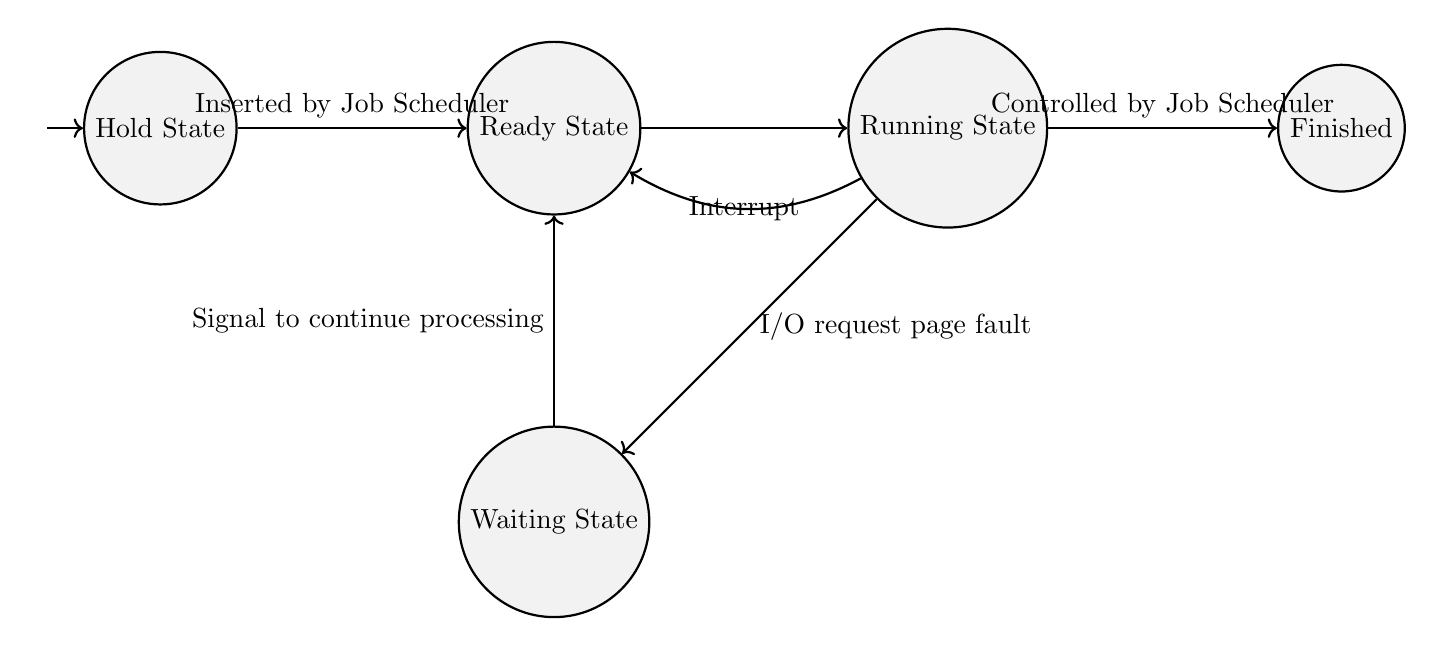
\begin{tikzpicture}[node distance={5cm},thick,main/.style = {draw, circle}]
    \node[state, initial] (hold) {Hold State};
    \node[state, right of=hold] (ready) {Ready State};
    \node[state, right of=ready] (run) {Running State};
    \node[state, below of=ready] (wait) {Waiting State};
    \node[state, right of=run] (fin) {Finished};

    \draw
    (hold) edge[above] node {Inserted by Job Scheduler} (ready)
    (ready) edge[above] node {} (run)
    (run) edge[above] node {Controlled by Job Scheduler} (fin)
    (wait) edge[left] node {Signal to continue processing} (ready)
    (run) edge[right] node {I/O request page fault} (wait)
    (run) edge[bend left] node {Interrupt} (ready)
    ;

  \end{tikzpicture}
  \caption{Job / Process State Diagram}
\end{figure}

When a job is accepted by the system it goes through the following states:

The job is put on HOLD and placed in a queue. In some systems the job
spooler / disk controller creates a table with the characteristics of
each job in the queue, and notes the important features of each job
such as estimated CPU time, priority, special I/O devices, required
and maximum memory required. This table is used by the Job Scheduler
to decide which job to run next.

Then the job moves to the READY state after the interrupts have been
resolved or placed on the READY queue directly in some systems. The
process then moves to RUNNING when the Process Scheduler allocates
CPU time to it. WAITING means the process can't continue until a
specific resource is allocated or an I/O operation as finished, and
then it can move back to READY. When the process is completed it
moves to the FINISHED state and is removed from the system.

Transitions from job statuses (HOLD $\to $ READY, RUNNING $\to $
FINISHED) are controlled by the Job Scheduler, while transitions
between process / thread statuses, i.e. all other transitions, are
controlled by the Process Scheduler.

\subsection{Thread States}
\begin{itemize}
  \item READY
  \item RUNNING
  \item WAITING
  \item DELAYED
  \item BLOCKED
\end{itemize}

Threads move through five states as they are processed by the system,
as shown in the state diagram below. When a process creates a thread
it is made ready by allocating to it the needed resources and placing
it in the READY queue. The thread state changes from READY to RUNNING
when the Process Scheduler assigns it to a processor.

\begin{figure}[htpb]
  \centering
  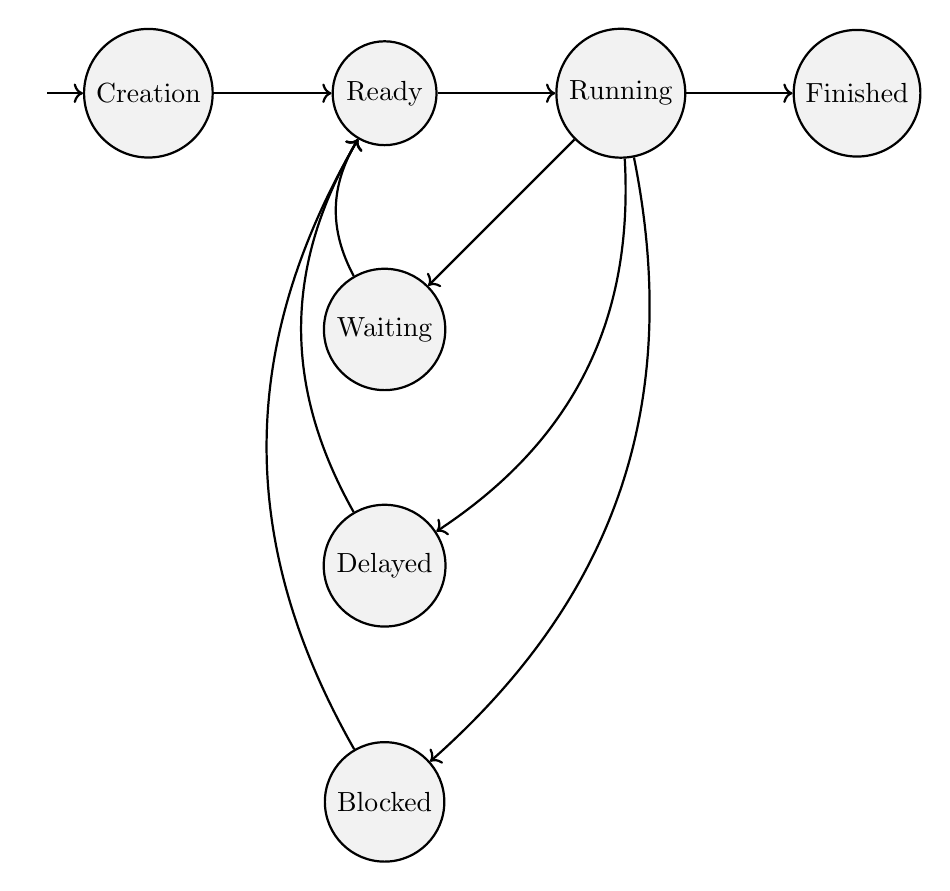
\begin{tikzpicture}[node distance={3cm},thick,main/.style = {draw, rectangle}]
    \node[state, initial] (create) {Creation};
    \node[state, right of=create] (ready) {Ready};
    \node[state, right of=ready] (run) {Running};
    \node[state, right of=run] (fin) {Finished};
    \node[state, below of=ready] (wait) {Waiting};
    \node[state, below of=wait] (delay) {Delayed};
    \node[state, below of=delay] (block) {Blocked};

    \draw
    (create) edge[above] node {} (ready)
    (ready) edge[above] node {} (run)
    (run) edge[above] node {} (fin)

    (run) edge[right] node {} (wait)
    (run) edge[bend left] node {} (delay)
    (run) edge[bend left] node {} (block)

    (wait) edge[bend left] node {} (ready)
    (delay) edge[bend left] node {} (ready)
    (block) edge[bend left] node {} (ready)
    ;

  \end{tikzpicture}
  \caption{Thread State Diagram}
\end{figure}

A thread can move from RUNNING to WAITING when it has to wait for an
event outside it's control to occur, like, an
input from the user, then back to READY when the event has occurred.
Alternatively another thread that is finished running can send a
signal indicating that the waiting thread can continue processing.

When an application has the ability to delay the processing of a
thread for some time, it causes the thread to move from RUNNING to
DELAYED. When the delay time has passed the thread moves from DELAYED
back to READY, for example the saving of a document every five minutes.

A thread moves from RUNNING to BLOCKED when an I/O request is issued.
After the I/O operation is done, the thread returns to the READY
state. When a thread is finished it moved to the FINISHED state and
all the allocated resources are deallocated.

\subsection{Control Blocks}
\dfn{Process Control Block (PCB)}{
  Contains information about each process in a system, including:
  \begin{itemize}
    \item Process Identifier (PID) - Unique Identifier assigned by
      the Job Scheduler
    \item Process Status - The current status of the job, i.e. READY,
      RUNNING, WAITING
    \item Process state - Contains all the information needed to
      indicate the current state of the job
      \begin{itemize}
        \item Process Status Word - The current instruction counter
          and register contents when the job isn't running but is
          either on HOLD, READY or WAITING.
        \item Register Contents - The contents of the register if the
          job has been interrupted and is waiting to resume processing.
        \item Main Memory - The address where the job is stored, and
          in the case of virtual memory, the linking between the
          virtual and physical memory locations.
        \item Resources - Information about all the resources
          allocated to this job, with each resources having an
          identification field listing its type, details of its
          allocation such as the sector address on a disk.
        \item Process Priority - Used by priority scheduling
          algorithms to select which job to run next.
      \end{itemize}
    \item Accounting Information - Information used for billing
      purposes and performance measurement.
  \end{itemize}
}

\dfn{Thread Control Block (TCB)}{
  Contains information about each thread in a system, including:
  \begin{itemize}
    \item Thread Identifier (TID) - Unique Identifier assigned by
      the Process Scheduler when the thread is created.
    \item Thread State - The current state of the thread, i.e. READY,
    \item CPU Information - Everything the operating system needs to know.
      \begin{itemize}
        \item Program Counter - How far the thread has progressed in
          its execution, and which instruction is currently being executed.
        \item Register Contents - The contents of the registers when the
          thread is not running.
      \end{itemize}
    \item Thread Priority - Used to indicate the weight of a thread
      relative to other thread. Determines which thread should be
      selected from the READY queue next.
    \item Pointer to process that created the thread - Indicates the
      process that created the thread.
    \item Pointers to all other threads created by this thread -
      Indicates child threads created by this thread.
  \end{itemize}
}

Each process in the system is represented by a Process Control
Block(PCB), and each thread is represented by a Thread Control
Block(TCB). These control blocks contain necessary management
information about the processes and threads, allowing the operating
system to manage them effectively.

The PCB is created when the Job Scheduler accepts the job and its
updated as the job progresses from the beginning to the end of the
its execution, while the TCB is created when a thread is created by a
process and updated as the thread progresses through its states.

Queues use control blocks to track jobs. As the job moves through the
system its progress is noted in the control block. This allows for
interrupted processes and threads to be resumed after a delay. The
control block is linked to other control blocks to form queues, for
example the READY queue.

\section{Scheduling Policies and Algorithms}

\dfn{Turnaround Time}{
  The total time taken between the submission of a process and its
  completion. It includes the time spent waiting to get into memory,
  waiting in the ready queue, executing on the CPU and doing I/O
  operations.
}

\dfn{Natural Wait}{
  The time a process spends waiting for I/O operations to complete.
}

\dfn{Pre-emptive Scheduling}{
  A scheduling strategy that interrupts the processing of a job and
  transfers the CPU to another job.
}

\dfn{Non-Pre-emptive Scheduling}{
  A scheduling strategy that allows a job to run until it completes or
  switches to the WAITING state.

}

In a multiprogramming environment, the operating system must decide
how to resolve three limitations of the system before scheduling
processes effectively:
\begin{itemize}
  \item There are a finite number of resources
  \item Some resources are non-shareable once allocated.
  \item Some resources require operator intervention to allocate or deallocate.
\end{itemize}

A good scheduling policy should aim to achieve the following goals,
even though some goals may contradict each other:
\begin{description}
  \item[Maximize Throughput]  - Run as many jobs as possible in a
    given amount of time.
  \item[Minimize Response Time ] - Quickly turn
    around interactive requests.
  \item[Minimize Turnaround time] - Move entire jobs in and out of
    the system quickly.
  \item[Minimize Waiting Time] - Move jobs out of the READY queue as
    quickly as possible.
  \item[Maximize CPU efficiency] - Keep the CPU busy 100\% of the time.
  \item[Ensure fairness for all jobs] - Give every job an equal
    amount of CPU and I/O time.
\end{description}

\section{Scheduling Algorithms}

\dfn{Scheduling Algorithm}{
  A set of rules that the operating system uses to allocate the CPU
  in the best way for moving jobs through the system efficiency.
}

\subsection{First-Come, First-Served (FCFS)}

A nonpreemtive scheduling algorithm that handles all incoming objects
according to their arrival time: The earlier they arrive the sooner
they're processed. This algorithm is commonly used for batch systems,
and is unacceptable for many interactive systems because interactive
users expect quick response time.

With FCFS as a new job enters the system, its PCB is placed at the
end of the READY queue, and when the CPU becomes available the job at
the front of the READY queue is selected for processing. In a strict
FCFS system there is no WAITING state because each job is run to its
completion, although there are many systems allowing context switches
on natural wait requests, with execution resuming when the I/O
operation is completed. Assuming there's no multiprogramming,
turnaround time is unpredictable with a strict FCFS policy, as each
jobs runs to completion so all other jobs must wait until the job is done.

\ex{}{
  Given the following jobs arrive in the order listed:
  \begin{itemize}
    \item Job A - 15 ms CPU time
    \item Job B - 2 ms CPU time
    \item Job C - 1 ms CPU time
  \end{itemize}

  If all three jobs arrive at time 0, the turnaround time (finish
  time $-$ arrival time) for each job is:
  \begin{align*}
    \text{Job A} &=  15 - 0 = 15 \\
    \text{Job B} &= 17 - 0 = 17 \\
    \text{Job C} &= 18 - 0 = 18 \\
  \end{align*}
  The average turnaround time is:
  \begin{align*}
    \frac{15 +  17 + 18}{3} &= 16.67  \\
  \end{align*}

  However if the jobs arrived in the order C, B, A, the turnaround times, are:
  \begin{align*}
    \text{Job C} &= 1 - 0 = 1 \\
    \text{Job B} &= 3 - 0 = 3 \\
    \text{Job A} &= 18 - 0 = 18 \\
  \end{align*}
  The average turnaround time is:
  \begin{align*}
    \frac{1 + 3 + 18}{3} &= 7.34  \\
  \end{align*}

}

Due to the unpredictability of turnaround times, the average
turnaround times are rarely minimized. If one job monopolizes the
system the effect on system performance depends on the type of job,
i.e. CPU bound or I/O bound. With a CPU bound job using the  CPU, the
other jobs in the system that are waiting for processing or finishing
I/O requests have to wait longer to for CPU time. If I/O requests are
not being serviced the I/O queue remain stable while the READY queue
grows with new arrivals, with extreme cases having the READY queue
filled to capacity while the I/O queue is empty.

On the other hand if an I/O bound job is using the CPU, the other
jobs in the system that are waiting for processing or finishing I/O
requests have to wait less time for CPU time. Since I/O bound jobs
frequently issue I/O requests, the I/O queue grows while the READY
queue shrinks as jobs complete their I/O requests and return to the
READY queue, leaving the CPU idle waiting for the next job to arrive.

\subsubsection{Key Points of FCFS}
\begin{itemize}
  \item Simple and easy to implement.
  \item Non pre-emptive
  \item Mostly used in batch systems.
  \item FIFO queue.
  \item Turnaround time is unpredictable and not minimized.
\end{itemize}

\subsection{Shortest Job Next (SJN) / Shortest Job First (SJF)  }

A nonpreemtive scheduling algorithm that chooses jobs based on the
length of their CPU cycle time. This algorithm works best in an
environment where the estimated CPU time required to run the job is
given in advance by each user at the start of the job, i.e. a batch
system. In interactive systems this information is not usually
available so SJN is not commonly used.

\ex{}{
  Given the following jobs all arriving at time 0:
  \begin{itemize}
    \item Job A - 5 CPU cycles
    \item Job B - 2 CPU cycles
    \item Job C - 6 CPU cycles
    \item Job D - 4 CPU cycles
  \end{itemize}

  The SJN algorithm would schedule the jobs with the shortest CPU
  cycles first, resulting in this order: B, D, A, C. This gives the
  following turnaround times:
  \begin{align*}
    \text{Job B} &= 2 - 0 = 2  \\
    \text{Job D} &= 6 - 0 = 6 \\
    \text{Job A} &= 11 - 0 = 11 \\
    \text{Job C} &= 17 - 0 = 17 \\
  \end{align*}
  Resulting in an average turnaround time of:
  \begin{align*}
    \frac{2 + 6 + 11 + 17}{4} &= 9 \\
  \end{align*}
}

The SJN algorithm consistently minimizes the average turnaround time
because the time for the first job has the biggest impact on the
average turnaround time as it affects the waiting time of all other
jobs in the READY queue. By executing the shortest jobs first, SJN
reduces the waiting time for all other jobs, leading to a lower
average turnaround time overall.

However SJN is only optimal if all jobs arrive at the same time, and
the CPU can accurately predict the CPU time required for each job.

\subsubsection{Key Points of SJN}
\begin{itemize}
  \item Simple and easy to implement.
  \item Non pre-emptive
  \item Mostly used in batch systems.
  \item Requires knowledge of CPU time required for each job.
  \item Minimizes average turnaround time.
  \item Only optimal if all jobs arrive at the same time and accurate
    CPU time predictions are available.
\end{itemize}

\subsection{Priority Scheduling}

Nonpreemtive algorithm that gives preference to important jobs based
on some criteria. Important jobs aren't interrupted until their CPU
cycles are completed or a natural wait occurs.  If two or more jobs
with equal priority are present in the READY queue, the processor is
allocated using FCFS.

Priorities can be assigned by a system administrator using extrinsic job
characteristics. With a priority algorithm job PCBs are usually
placed at the end of one of several READY queues by the Job Scheduler
based on their priority so that the Process Scheduler manages
multiple READY queues. Some intrinsic characteristics that can be
used to assign priorities include:
\begin{description}
  \item[Memory Requirements]  - Jobs requiring large amounts of
    memory could have lower priorities, or vice versa.
  \item[Number and type of I/O devices] - Jobs requiring many I/O
    devices could be given lower priorities, than those requiring few
    I/O devices.
  \item[Total CPU time] - Jobs having a long CPU cycle or estimated
    run time could be given lower priorities, than those with short CPU cycles.
  \item[Amount of time already spent in the system] - Some systems
    increase the priority of jobs that have been in the system for an
    unusually long time to prevent starvation. This is called \textbf{ageing}.
\end{description}

\subsubsection{Key Points of Priority Scheduling}
\begin{itemize}
  \item Non pre-emptive
  \item Can be used in both batch and interactive systems.
  \item Requires knowledge of job characteristics to assign priorities.
  \item Can lead to starvation of low-priority jobs.
\end{itemize}

\subsection{Shortest Remaining Time (SRT)}

A preemptive version of the SJN algorithm, that allocates jobs
closest to completion, allowing new jobs with shorter remaining times
to interrupt running jobs. When using SRT if several jobs have the
same amount of time remaining the algorithm falls back to FCFS.

This algorithm cannot be implemented in an interactive system because
it requires knowledge of the exact CPU time required to finish each
job, which is only available in batch systems. SRT involves more
overhead than SJN in the form of context switching and monitoring of
remaining times.

\ex{}{
  Given the following jobs:
  \begin{itemize}
    \item Job A - 6 ms CPU time, arrives at time 0
    \item Job B - 3 ms CPU time, arrives at time 1
    \item Job C - 1 ms CPU time, arrives at time 2
    \item Job D - 4 ms CPU time, arrives at time 3
  \end{itemize}
  The finish times for each job using SRT are:
  \begin{itemize}
    \item Job A - Starts at time 0, interrupted at time 1, resumes at
      time 9, finishes at time 14
    \item Job B - Starts at time 1, interrupted at time 2, resumes at
      time 3, finishes at time 5
    \item Job C - Starts at time 2, finishes at time 3
    \item Job D - Starts at time 5, finishes at time 9
  \end{itemize}
  For each job the turnaround time is:
  \begin{align*}
    \text{Job A} &= 14 - 0 = 14  \\
    \text{Job B} &=  5 - 1 = 4 \\
    \text{Job C} &= 3 - 2 = 1 \\
    \text{Job D} &=  9 - 3 = 6 \\
  \end{align*}
  Resulting in an average turnaround time of:
  \begin{align*}
    \frac{14 + 4 + 1 + 6}{4} &= 6.25 \\
  \end{align*}
}

SRT is often affected by the time needed for context switching, especially if
many jobs with short remaining times arrive frequently, causing
numerous interruptions. How context switching is done depends on the
CPU architecture, which the overhead depending on the way the CPU
handles interrupts. Although SRT appears to be faster, in a real
operating environment its advantages may be negated by the time spent
context switching.

\subsubsection{Key Points of SRT}
\begin{itemize}
  \item Pre-emptive
  \item Mostly used in batch systems.
  \item Requires knowledge of CPU time required for each job.
  \item Minimizes average turnaround time.
  \item Affected by context switching overhead.
\end{itemize}

\subsection{Round Robin (RR)}
A preemptive scheduling algorithm, used in interactive systems, that
allocates CPU time to each job in a FCFS manner for a fixed time
period called a \textbf{time quantum} or \textbf{time slice}.

Jobs are placed in the READY queue using a FIFO structure, with the
job at the front of the queue being allocated the CPU for a time
quantum. If processing isn't finished when the time quantum expires,
the job is interrupted and put at the end of the READY queue, with
it's information saved in its PCB. The next job in the READY queue is
then allocated the CPU for a time quantum, and this process continues
until all jobs are completed.

If the job's CPU cycle is smaller than the time quantum one of two
actions can take place:
\begin{itemize}
  \item If this is the job's last CPU cycle and the job is finished,
    then all resources allocated to it are released and the completed
    job is returned to the user.
  \item If the CPU has been interrupted by an I/O request, then the
    information about the job is saved in its PCB and the job is
    placed in the WAITING queue. When the I/O operation is completed
    the job is placed at the end of the READY queue.
\end{itemize}

\ex{}{
  Given the following jobs:
  \begin{itemize}
    \item Job A - 8 ms CPU time, arrives at time 0
    \item Job B - 4 ms CPU time, arrives at time 1
    \item Job C - 9 ms CPU time, arrives at time 2
    \item  Job D - 5 ms CPU time, arrives at time
  \end{itemize}
  With a time quantum of 4 ms, the finish times for each job using RR are:
  \begin{itemize}
    \item Job A - Starts at time 0, interrupted at 4, resumes at 16 and
      finishes at time 20
    \item Job B - Starts at time 4, interrupted at time 8, finishes at time 8
    \item Job C - Starts at time 8, interrupted at time 12, resumes
      at time 20, and is interrupted at time 24, resumes at time 25 and
      finishes at time 26
    \item Job D - Starts at time 12, interrupted at time 16, resumes
      at time 24 and
      finishes at time 25
  \end{itemize}
  For each job the turnaround time is:
  \begin{align*}
    \text{Job A} &= 20 - 0 = 20 \\
    \text{Job B} &= 8 - 1 = 7 \\
    \text{Job C} &=26 - 2 = 24 \\
    \text{Job D} &= 25 - 3 = 22 \\
  \end{align*}
}

The length of the time quantum is critical to the performance of the RR
algorithm. If the system is a time-critical system requiring low
response times, then the time quantum should be small allowing jobs
to be processed quickly. If it's an archival system, turnaround time
and overhead become critically important, so a larger time quantum is preferred.

The general rules for selecting a time quantum are:
\begin{enumerate}
  \item It should be long enough to allow 80\% of the CPU cycles to
    run to completion
  \item It should be at least 100 times longer than the time required
    to perform one context switch.
\end{enumerate}

\subsubsection{Key Points of RR}
\begin{itemize}
  \item Pre-emptive
  \item Mostly used in interactive systems.
  \item Time quantum critical to performance.
  \item Provides good response time.
  \item Can lead to high turnaround time and overhead if time quantum
    is too small.
\end{itemize}

\subsection{Multiple-Level Queues (MLQ)}

Multiple-Level queues isn't a specific scheduling algorithm, but
works in conjunction with several schemes to handle jobs that can be
grouped according  to one or more common characteristics. An example
is the priority scheduling algorithm where jobs are grouped according to
their priority levels.

Another approach is to group jobs according to their processing
characteristics, i.e. CPU bound or I/O bound, with the Process
Scheduler alternating between jobs from each group to keep the system
balanced ensuring that neither CPU nor I/O devices are idle for long periods.

Another example would be a preemptive approach in a hybrid
environment where batch jobs are put into one queue, the background
queue, and interactive jobs are put into another queue, the
foreground queue. The jobs in the foreground queue are given higher
priority, focusing on faster turnaround, than those in the background queue.

There are four primary methods for determining movement:
\begin{itemize}
  \item No Movement Between Queues
  \item Movement Between Queues
  \item Variable Time Quantum Per Queue
  \item Ageing
\end{itemize}

\subsubsection{No Movement Between Queues}

A simple policy that works best with high priority jobs. The
processor is allocated to the jobs in the highest priority queue in a
FCFS manner until the queue is empty, then the next highest priority
queue is processed, and so on. This policy works best when there are
relatively free users with hight priority jobs so that the top queues
quickly empty out, allowing the processor to spend most of its time
processing lower priority jobs.

\subsubsection{Movement Between Queues}

A policy that adjusts the priorities assigned to each job. High
priority jobs are treated like all others once they enter the system,
allowing them to move between queues based on their behaviour. When a
time quantum interrupt occurs the job is moved to the end of the next
lower priority queue, and so on. A job can also have its priority
increased in cases when it issues an I/O request before its time
quantum expires, moving it to the end of the next higher priority queue.

This policy works best in a system where jobs are handled according
to  their computing cycle characteristics, i.e. CPU bound or I/O
bound. This assumes that a job that exceeds its time quantum is CPU
bound and will require more CPU time than one that requests I/O
before the time quantum expires. There fore the CPU-bound jobs are
placed at the end of the next lower-level queue when they're
interrupted because of the time quantum expiring, while I/O bound
jobs are returned to the end of the next higher-level queue once
their I/O request has finished. This facilitates I/O-bound jobs and
works well for interactive systems.

\subsubsection{Variable Time Quantum Per Queue}

A variant of the movement between queues policy, allowing faster
turnaround for CPU-bound jobs. Each queue is given a time quantum
twice as long as the one before it. For example if the highest
priority queue has a time quantum of 100 ms, the next lower priority
queue has a time quantum of 200ms, and so on.

If a job doesn't finish its CPU cycle using the first time quantum,
it is moved to the end of the next lower-level queue, and when the
processor is next allocated to it the job is allowed to execute for
longer and longer periods of time, thus improving its chances of
finishing in a reasonable amount of time.

\subsubsection{Ageing}

\dfn{Starvation}{
  A situation where a low-priority job is perpetually denied access
  to the CPU because higher-priority jobs keep arriving.
}

Used to ensure that jobs in the lower-level queues will eventually
complete their execution. The operating system keeps track of each
job's waiting time, and when a job gets too old, i.e. when it has
waited in the queues for so long that it has reached a certain time
limit, the system moves the job into the next highest queue and so
on, until it reaches the highest priority queue. Ageing prevents
indefinite postponement of low-priority jobs, ensuring that all jobs
eventually get processed. Eventually the situation could lead to the
old job's starvation, causing it to never be processed. This poses a
significant threat to a system if the job is allocated critical resources.

\subsection{Earliest Deadline First (EDF)}
A Dynamic preemptive priority algorithm used to address the critical
processing requirements of real-time systems and their deadlines.
With EDF the priority of a job can be adjusted as the job moves
through execution from START to FINISHED.

The goal of EDF is to process all jobs in the order that is most
likely to allow each to run to completion before reaching their
respective deadlines. Initially jobs are assigned priorities based on
the amount of time remaining until the job's impending deadline, i.e.
inversely proportional to its absolute deadline. Therefore the closer
the deadline, the higher the priority. As new jobs arrive or existing
jobs complete, the priorities are recalculated to ensure that the job
with the nearest deadline is always given precedence, and if two or
more jobs have the same deadline, the job that arrived first is given priority.

\ex{}{
  Given the following jobs:
  \begin{itemize}
    \item  Job A - 3 ms CPU time, arrives at time 0, deadline at 6
    \item Job B - 1 ms CPU time, arrives at time 2, deadline at 2
    \item  Job C - 5 ms CPU time, arrives at time 2, deadline at j
  \end{itemize}
}

\section{Managing Interrupts}

\dfn{Interrupt Handler}{
  A control program that handles the interruption sequence of events
  when an interrupt occurs.
}

Interrupts can be sent by many events including:
\begin{itemize}
  \item Page faults
  \item I/O requests
  \item Timer expirations
  \item Illegal arithmetic operations
  \item Illegal job instructions
\end{itemize}

Interrupts are handled by the interrupt handler, when operation
system detect an error that is not recoverable, the interrupt handler
typically follows this sequence:
\begin{enumerate}
  \item The type of interrupt is described and stored to be passed on
    to the user as an error message.
  \item The state of the interrupted process is saved, including the
    value of the program counter, the mode specification, and the
    contents of all registers.
  \item  The interrupt is processed:
    \begin{itemize}
      \item The error message and the state of the of the interrupted
        process are sent to the user
      \item The program execution is halted
      \item Any resources allocated the job are released
      \item And the job exits the system.
    \end{itemize}
  \item The process resumes normal operation.
\end{enumerate}

However if he interrupt is nonrecoverable the job is terminated in Step 3.

\chapter{Process Synchronization}

\section{Consequences of Poor Synchronization}

\dfn{Deadlock}{
  A system-wide tangle of resource requests that begins when two or
  more jobs are put on hold, each waiting for a vital resource to be
  become available, but if the resources needed by those jobs are the
  resources held by the other jobs in the deadlock, none of the jobs
  can proceed. The deadlock is complete if the remainder of the
  system comes to a halt too.
}

\dfn{Race} {
  A synchronization problem between two or more processes vying for
  the same resource.
}

\dfn{Race Condition}{
  A situation where the outcome of a program depends on the relative
  timing of events that are not explicitly controlled by the program.
}

Fixing deadlocks is critical to maintaining system stability and
performance. Deadlocks can lead to several negative consequences,
including:
\begin{description}
  \item[Starvation]  - Low-priority jobs may never get access to
    resources if higher-priority jobs keep arriving.
  \item[Reduced System Throughput]  - Deadlocks can lead to a
    significant reduction in system throughput as resources are
    tied up in deadlocked processes, preventing other processes from
    executing.
  \item[Increased Response Time]  - Deadlocks can lead to increased
    response times for processes as they wait for resources to
    become available.
\end{description}

\section{Examples of Deadlocks}

A deadlock can occur when a nonshareable  and nonpreemtive resources,
such as printers or scanners, are allocated to jobs that eventually
require other nonshareable, nonpreemtive resources that have been
allocated to other jobs.

\subsection{Deadlocks on File Requests}

If jobs are allowed to request and hold files for the duration of
their execution a deadlock can occur. In this case each job holds one
file and requests another file held by another job. For example Job A
holds File 1 and requests File 2, while Job B holds File 2 and
requests File 1. Neither job can proceed because each is waiting for a
file held by the other job, resulting in a deadlock.

\subsection{Deadlocks in Databases}

A deadlock can also occur if two process access and lock records in a
database. For example Process A locks Record 1 and requests
Record 2, while Process B locks Record 2 and requests Record 1. Neither
process can proceed because each is waiting for a record locked by the
other process, resulting in a deadlock.

\subsection{Deadlocks in Dedicated Device Allocation}

\subsection{Deadlocks in Multiple Device Allocation}

\subsection{Deadlocks in Spooling}

\subsection{Livelock while Disk Sharing}

\dfn{Livelock}{
  A situation where two or more processes continuously change their
  state in response to changes in the other processes without making
  any progress.
}

\section{Necessary Conditions of Deadlocks}

In each example of deadlock/livelock, there was some interaction of
several processes and resources but each time, it was preceded by the
simultaneous occurrence of four conditions that the operating system
could have recognized:
\begin{description}
  \item[Mutual Exclusion]  - At least one resource must be held in a
    nonshareable mode, meaning that only one process can use the
    resource at any given time.
  \item[Resource Holding]  - A process must be holding at least one
    resource and waiting to acquire additional resources that are
    currently being held by other processes.
  \item[No Preemption]  - Resources cannot be forcibly removed from
    processes holding them until the resources are used to
    completion.
  \item[Circular Wait]  - A set of processes must exist such that
    each process is waiting for a resource that is held by the next
    process in the chain, forming a circular chain of processes
    where each process is waiting for a resource held by the next
    process.
\end{description}

All four conditions must hold simultaneously for a deadlock to occur,
and as long as these four conditions persist, the deadlock will
persist. So if one condition is removed the deadlock will be
resolved, in fact if the four conditions can be prevented from ever
occurring simultaneously then deadlocks can be completely avoided.

\section{Strategies for Handling Deadlocks}
\begin{itemize}
  \item Prevention - Prevent occurrence of one condition.
    \begin{itemize}
      \item Mutual Exclusion - Some resources must allocate
        exclusively. Bypassed if I/O device uses spooling.
      \item  Resource Holding
        \begin{itemize}
          \item Bypassed if jobs request every necessary resource at
            creation time.
          \item  Multiprogramming degree significantly decreased
          \item  Idle peripheral devices
        \end{itemize}

    \end{itemize}
  \item  Avoidance - Avoid deadlock if it becomes probable.
  \item Detection - Detect deadlock when it occurs.
  \item  Recovery - Resume in a graceful manner.
\end{itemize}

Generally operating systems use a combination of several strategies
to deal with deadlocks.
\begin{description}
  \item[Prevention] - Preventing deadlocks by ensuring that at least
    one of the necessary conditions cannot hold.
  \item[Avoidance] - Avoiding deadlocks by careful resource allocation
    based on knowledge of future resource requests.
  \item[Detection] - Detecting deadlocks when they occur using
    algorithms that periodically check the system for deadlocks.
  \item[Recovery] - Recovering from deadlocks by terminating or
    rolling back one or more processes involved in the deadlock.
\end{description}

\subsection{Prevention}

To prevent a deadlock the operating system must eliminate one of the
four necessary conditions for deadlock, further complicated by the
fact that the same conditions can't be eliminated from every resource.

\dfn{Spooling}{
  A process where data is temporarily gathered and stored to be
  accessed and processed by a device, program or the user at a later
  time.
}

Mutual exclusion is necessary in any computer system because some
resources, such as memory, CPU, and dedicated drivers, must be
exclusively allocated to one user at a time. In the case of I/O
devices such, the mutual exclusion may be bypassed by spooling which
allows the output from many jobs to be stored in separate temporary
spool files tat the same time, and each complete output file is then
selected for use when the I/O device becomes available. However this
solution may trade one problem (Deadlock in Device Allocation) for
another (Deadlocks in Spooling).

Resources holding can be resolved by forcing each job to request
every resource it will need to run to completion at the time of its creation.
This would significantly decrease the degree of multiprogramming in the system
because many resources would be tied up waiting for jobs to complete,
and I/O devices would be idle much of the time.

No preemption could be bypassed by allowing the operating system to
deallocate resources from jobs, using context switching to save the
current state of the job. This approach would also require complex
recovery tasks in the cause of the preemption of a dedicated I/O
resource, or files modified by the job.

Circular wait can be resolved if the operating system prevents the
formation of a circular chain of processes. This can be done by
numbering the available resources
in a system and requiring that each job requests resources in
ascending order, i.e. a job holding Resource 1 can only request
Resource 2, 3, and so on, This removes the possibility of a circular
wait preventing deadlocks. However this approach may lead to long
idle times for unused resources allocated in the lower numbers.

\subsection{Avoidance}

The operating system can avoid deadlocks if the system knows ahead of
time the sequence of requests associated with each of the active processes.

The Banker's Algorithm proposed by Dijkstra (1965) can be used to
regulate resource allocation to avoid deadlocks. It is based on a
bank with a fixed amount  of capital that operates on the following principles:
\begin{itemize}
  \item No customer will be granted a loan exceeding the bank's total capital.
  \item All customers will be given a maximum credit limit when
    opening an account.
  \item No customer will be allowed to borrow over the limit.
  \item The sum of all loans won't exceed the bank's total capital.
\end{itemize}

To remain in a safe state the bank must ensure it has sufficient
funds to satisfy at least one customer.

\ex{}{
  Given a system with 10 resources available and three processes,
  with the following maximum resource requirements:
  \begin{table}[H]
    \begin{center}
      \begin{tabular}{|c c c c|}
        \hline
        Job No. & Devices Allocated & Maximum Required & Remaining
        Needs \\ [0.5ex]
        \hline
        \hline
        1 & 0 & 4 & 4 \\
        2 & 2 & 5 & 3 \\
        3 & 4 & 8 & 4 \\
        \hline
        Total number of devices allocated = 6 & & & \\
        \hline
        Total number of devices in system = 10 & & & \\
        \hline
        Available devices = 4 & & & \\
        \hline
      \end{tabular}
    \end{center}
  \end{table}

  This is a \textbf{safe state} because available devices (4) $\geq$
  smallest remaining need (3 for Job 2), so at least one job can complete.

  The OS allocates more resources to Jobs 1 and 2 and enters an unsafe state:
  \begin{table}[H]
    \begin{center}
      \begin{tabular}{|c c c c|}
        \hline
        Job No. & Devices Allocated & Maximum Required & Remaining
        Needs \\ [0.5ex]
        \hline
        \hline
        1 & 2 & 4 & 2 \\
        2 & 3 & 5 & 2 \\
        3 & 4 & 8 & 4 \\
        \hline
        Total number of devices allocated = 9 & & & \\
        \hline
        Total number of devices in system = 10 & & & \\
        \hline
      \end{tabular}
    \end{center}
  \end{table}

  This state is \textbf{unsafe} because with only one device
  available, the system
  can't satisfy anyone's minimum remaining needs (all jobs need at
  least 2 devices).
  If the system allocated the last resource to any process, it would enter a
  deadlock because it wouldn't be able to satisfy the remaining needs
  of any process. An unsafe state doesn't necessarily lead to
  a deadlock, but it does indicate the possibility of one occurring.

  The operating system must never satisfy a request that moves it
  from a safe state to an unsafe state. Therefore, as user's requests
  are satisfied, the OS must identify the job with the smallest number
  of remaining resources and make sure that the number of available
  resources is always equal to or greater than the number needed for
  this job to run to completion.

  The correct sequence of resource allocation to keep the system in a safe
  state is as follows:

  \textbf{Step 1:} Starting from the initial safe state, allocate 3
  resources to Job 2 (smallest remaining need):
  \begin{table}[H]
    \begin{center}
      \begin{tabular}{|c c c c|}
        \hline
        Job No. & Devices Allocated & Maximum Required & Remaining
        Needs \\ [0.5ex]
        \hline
        \hline
        1 & 0 & 4 & 4 \\
        2 & 5 & 5 & 0 \\
        3 & 4 & 8 & 4 \\
        \hline
        Total number of devices allocated = 9 & & & \\
        \hline
        Total number of devices in system = 10 & & & \\
        \hline
      \end{tabular}
    \end{center}
  \end{table}

  Job 2 completes and releases all 5 devices. Available devices = 1 + 5 = 6.

  \textbf{Step 2:} Allocate 4 resources to Job 1:
  \begin{table}[H]
    \begin{center}
      \begin{tabular}{|c c c c|}
        \hline
        Job No. & Devices Allocated & Maximum Required & Remaining
        Needs \\ [0.5ex]
        \hline
        \hline
        1 & 4 & 4 & 0 \\
        2 & \textit{finished} & -- & -- \\
        3 & 4 & 8 & 4 \\
        \hline
        Total number of devices allocated = 8 & & & \\
        \hline
        Total number of devices in system = 10 & & & \\
        \hline
      \end{tabular}
    \end{center}
  \end{table}

  Job 1 completes and releases all 4 devices. Available devices = 2 + 4 = 6.

  \textbf{Step 3:} Allocate 4 resources to Job 3:
  \begin{table}[H]
    \begin{center}
      \begin{tabular}{|c c c c|}
        \hline
        Job No. & Devices Allocated & Maximum Required & Remaining
        Needs \\ [0.5ex]
        \hline
        \hline
        1 & \textit{finished} & -- & -- \\
        2 & \textit{finished} & -- & -- \\
        3 & 8 & 8 & 0 \\
        \hline
        Total number of devices allocated = 8 & & & \\
        \hline
        Total number of devices in system = 10 & & & \\
        \hline
      \end{tabular}
    \end{center}
  \end{table}

  Job 3 completes and releases all 8 devices. All jobs have completed
  successfully.

  The safe sequence is: \textbf{Job 2 $\rightarrow$ Job 1 $\rightarrow$ Job 3}.
}

In implementing the Banker's Algorithm the system must setup  a
resource assignment table for each type of resource, and tracks each
table to keep the system in a safe state.

Although the Banker's Algorithm can effectively avoid deadlocks, it
has several limitations:
\begin{itemize}
  \item  As jobs enter the system they must declare the maximum
    number of resources they need, which is difficult in interactive systems.
  \item The number of total resources for each class must remain
    constant. If a device fails and becomes unavailable the algorithm
    may no longer be able to keep the system in a safe state.
  \item The number of jobs must remain fixed, which is hard to do in
    an interactive system.
  \item High overhead as the algorithm must be executed each time a
    jobs requests a resource.
\end{itemize}

\subsection{Detection}

Deadlock detection can be modelled as a directed graph problem,
allowing use of cycle detection algorithms to identify deadlocks.
Unlike avoidance algorithms which must be executed on each request,
cycle detection algorithms can be executed when appropriate, i.e.
every hour, once a day, or manually by the system administrator.

Beginning with a system in use, the steps to detect deadlocks are:
\begin{enumerate}
  \item Find a process that is currently using a resource and waiting
    for one . This process can be removed from the graph by
    disconnecting the link tying the resource to the process. The
    resource can then be returned to the available list. This is
    possible because the process would eventually finish and return
    the resource.
  \item Find a process that's waiting only for resources classes that
    aren't fully allocated. This process isn't contributing to
    deadlock since it would eventually get he resource it's waiting
    for, finish it's work and return the resource at he available list.
  \item Repeat step 1 and continue with steps 1 and 2 until all the
    lines connect resources to processes have been removed.
\end{enumerate}

If there are any edges left in the graph this indicates that request
of the process in question can't be satisfied and the process is deadlocked.

\subsection{Recovery}

Once a deadlock is detected it must be resolved and the system
returned to normal as quickly as possible. There are several recovery
algorithms but they all have a common approach: sacrificing at least
one victim, i.e. an expendable job, which when removed from the
deadlock, will free the system. Removal generally involves restarting
the job from the beginning or from a previously saved checkpoint.

The first approach is to terminate every job that's active in the
system and restart them from the beginning. This is a simple approach
but is drastic and results in significant loss of processing time.

The second approach is to terminate only the jobs involved in the
deadlock and ask their users to resubmit them. This approach is less drastic but
still results in significant loss of processing time for the
terminated jobs.

The third approach is to identify which jobs are involved in the
deadlock and terminate them one at a time, checking to see if the
deadlock is resolved after each removal, until the deadlock is
resolved. This approach minimizes the number of jobs terminated but
requires more overhead to check for deadlock after each removal.

The fourth approach can be used only if the job keeps a record or a
checkpoint of its progress so it can be interrupted and continued
without starting again from the beginning of its execution.

The following methods focus on the non-deadlocked jobs and the
resources they hold

The fifth approach is to select a non-deadlocked job, then preempt
the resources it's holding, and allocate them to deadlocked process
so they can resume execution, resolving the deadlock. This
approach requires the ability to preempt resources, which may not be
possible for all resource types.

The sixth method stops new jobs from entering the system, allowing
the non-deadlocked jobs to finish so they'll release their resources
to the deadlocked jobs. This approach is the only one listed that
doesn't require a sacrifice. This method can be effective if the
deadlock involves only a few jobs and the non-deadlocked jobs will
finish in a reasonable amount of time, and is not guaranteed to work
unless the number of availiable resources is greater than the number
needed by at least one of the deadlocked jobs.

Several factors must be considered when selecting a sacrifice that
will have the least-negative effect on the system, including:
\begin{description}
  \item[Priority]  - High priority jobs are usually not sacrificed.
  \item[CPU time used] - Jobs close to completion are usually not sacrificed.
  \item[Number of releated jobs] - Jobs with many related jobs are
    usually not sacrificed.
\end{description}

\section{Starvation}

\dfn{Starvation}{
  A single job is prevented from completing its execution because it
  is waiting for resources that never become available.
}

Starvation can occur in systems that use priority scheduling, and can
have the following consequences:
\begin{description}
  \item[Increased Response Time] - Starvation can lead to increased
    response times for low-priority jobs as they wait indefinitely
    for resources to become available.
  \item[Reduced System Throughput] - Starvation can lead to a
    reduction in system throughput as low-priority jobs are unable to
    complete their execution.
  \item[Unfair Resource Allocation] - Starvation can lead to unfair
    resource allocation, where high-priority jobs are given
    preferential treatment over low-priority jobs.
\end{description}

To address this problem an algorithm can be used to track how long
each job has been waiting for resources, the same as \textbf{ageing}.
Once starvation has been detected, the system can block incoming
requests from other jobs until the starving jobs have been satisfied.

\chapter{Concurrent Processing}

\section{Parallel Processing}

\dfn{Parallel Processing}{
  The simultaneous operation and execution of two or more processors
  in one system
  at the same time.
}

The processor manager coordinates the activities of each processor,
and synchronizes interaction among CPUS. This allows for increased
reliability, as there is failover capability if one processor fails,
and faster processing as instructions can be executed in parallel
across multiple processors.

Processing can be done in several ways:
\begin{itemize}
  \item Each CPU could be allocated to each program or job
  \item Each CPU could be allocated to each working set or parts of it.
  \item Each individual instruction could be subdivided with each
    subdivision processed simultaneously
\end{itemize}

However there are challenges in parallel processing:
\begin{itemize}
  \item Connecting processors into configurations that allow efficient
    communication among them.
  \item Orchestrating processor interaction
\end{itemize}

\subsection{Levels Of Multiprocessing}

Multiprocessing can occur at three levels:
\begin{description}
  \item[Job Level]  - Several jobs are processed simultaneously,
    each job allocated to a different processor. No explicit synchronization.
  \item[Process Level]  - Several processes within a job are
    processed simultaneously, each process allocated to a different
    processor. Some level of synchronization.
  \item[Thread Level] - Several threads within a process are processed
    simultaneously, each thread allocated to a different processor.
    High degree of synchronization needed to track each process and each thread.
\end{description}

\subsection{Multi-Core Processors}

\dfn{Multi-Core Processor}{
  A single computing component (chip) with two or more independent
  processing units called cores, which read and execute program
  instructions.
}

Multi-core processors suffer from current leakage (tunnelling) as a
result of the
small size of the transistors used to build them. This leakage causes
increased power consumption and heat generation, which can lead to
reduced performance and reliability. To mitigate these issues,
multi-core processors often
reduce the speed of groups of adjacent cores when they are in use at
the same time to reduce heat generation.

\section{Typical Multiprocessing Configurations}

The configuration of multiple processors in a system affects how they
communicate and synchronize with each other. There are three typical
configurations:
\begin{itemize}
  \item Master / Slave Configuration
  \item Loosely Coupled Configuration
  \item Symmetric Configuration
\end{itemize}

\subsection{Master / Slave Configuration}
An asymmetric multiprocessing configuration where one processor/core
is designate as a master processor and all the others are designated
as slave processors managed by the master.
The master processor is responsible for
\begin{itemize}
  \item Managing the system
  \item Maintaining the status of all processes
  \item Managing storage
  \item Schedules work for other processors
  \item Executes control programs
\end{itemize}

This configuration is simple to implement and manage.

However it has several disadvantages:
\begin{description}
  \item[Reliability] - If the master processor fails the entire system
    may become inoperable.
  \item[Poor Resources Usage] - As slave processors may be idle
    while waiting for the master to allocate work to them.
  \item[Increased Interrupts] - The master processor may become
    overwhelmed with interrupts from slave processors requesting
    work or reporting status.
\end{description}

\subsection{Loosely Coupled Configuration}
Several processors each manage their own resources, with each
processor communicating and cooperating with others as needed.

This configuration requires several policies for job scheduling and
conditions. There is failover capability if one processor fails, and
processors can be added or removed
from the system as needed however failure is difficult to detect.

This configuration has several disadvantages:
\begin{description}
  \item[Requires Several Resouces] - Each processor must have its own memory
    and I/O devices, increasing the cost of the system.
  \item[Complex Communication] - Processors must communicate over a
    network, which can be slow and unreliable.
  \item[Complex Synchronization] - Processors must synchronize their
    activities, which can be difficult to implement.
\end{description}

\subsection{Symmetric Configuration}

All processors share resources and communicate with each other with
decentralized processor scheduling, where each processor uses the
same scheduling algorithm.

This configuration has several advantages:
\begin{description}
  \item[Relaiblity] -  If one processor fails, the others can continue
    to operate.
  \item[Efficient Resource Usage] - Processors can share resources,
    reducing idle time.
  \item[Load Balancing] - Work can be distributed evenly among processors,
    improving performance.
  \item[Graceful Degradation] - The system can continue to operate at a reduced
    capacity if one or more processors fail.
\end{description}

However it has several disadvantages:
\begin{description}
  \item[Difficult to Implement]  - Requires synchronization to
    prevent race conditions, deadlocks, and starvation.
  \item[Increased Overhead] - Due to the need for interrupt
    processing and updating process lists.
  \item[More Conficts] - As several processors access shared resources
    simultaneously.
\end{description}

\section{Process Synchronization Software}

\dfn{Critical Region / Section }{
  A part of a program that accesses a shared resource (data structure,
  file, device) that must not be concurrently accessed by more than one
  thread of execution.
}

To achieve process synchronization shared resources must be locked to
indicate use by another process to prevent conflicts, and only when
the resource is released can waiting processes access it.

Mistakes in synchronization can result in starvation, as jobs are
left waiting indefinitely and deadlock if two or more jobs are
waiting for resources held by each other.

In synchronization a critical region must be defined for each shared
resource, allowing only one process to access the resource at a time.
Processes within this critical region cannot be interleaved as this
threatens the integrity of the operation.

Synchronization can be implemented as a lock-and-key arrangement,
where processes determine key availability, i.e. if a process can
enter the critical region or must wait. If a process wants to enter a
critical region it must first obtain a key to gain access, this makes
the key unavailable to other processes until the process leaves the
critical region and releases the key.

There are three types of locking mechanisms:
\begin{itemize}
  \item Test-and-Set
  \item WAIT and SIGNAL
  \item Semaphores
\end{itemize}

\subsection{Test-and-Set}

\dfn{Atomic}{
  An instruction that runs to completion without the possibility of
  interruption.
}

An atomic instruction that checks if a key is available, and if
it is acquires it all in a single cycle. The key can be represented
as a single bit in a storage location with zero indicating the key is
available and one indicating the key is unavailable.

Before a process enters a critical region, it executes the
test-and-set (TS) instruction
if there is no process in the critical region, the TS instruction
sets the key to
one and allows the process to enter, when the process leaves the
critical region it
sets the key back to zero, allowing other processes to enter.

This approach has several advantages:
\begin{itemize}
  \item Simple to implement
  \item  Works well for a small number of processes
\end{itemize}

And several disadvantages:
\begin{description}
  \item[Starvation]  - Many processes may be waiting to enter a
    critical region as processes gain access arbitrarily.
  \item[Busy Waiting] - Waiting processes remain in unproductive,
    resource-consuming wait loops.
\end{description}

\subsection{WAIT and SIGNAL}

Improves upon test and set by removing busy waiting. This introduces
two mutually exclusive operations:
\begin{description}
  \item[WAIT]  - Activated when a process encounters the busy
    condition code. The
    process is placed in a waiting queue until the condition code is cleared.
  \item[SIGNAL] - Activated when process exits the critical region
    and the condition code is cleared. If there are processes in the
    waiting queue, one is removed and allowed to enter the critical region.
\end{description}

\subsection{Semaphores}

A non-negative integer variable access through atomic operations used
to indicate the status of a resource. It uses two atomic operations:
\begin{description}
  \item[P (Proberen)] - Tests the semaphore value, if it's greater
    than zero it decrements the value and allows the process to enter
    the critical region. If the value is zero the process is placed in
    a waiting queue until the value becomes greater than zero.
  \item[V (Verhogen)] - Increments the semaphore value when a process
    exits the critical region. If there are processes in the waiting
    queue, one is removed and allowed to enter the critical region.
\end{description}

A semaphore with vale 0 indicates that the resource is unavailable,
so the process calling the P operation is placed in the waiting
queue, and must wait until the value is greater than 0. In this way a
semaphore can allow multiple restricted access to a certain number of
processes simultaneously by initializing the semaphore to the number
of allowed processes.

This ensures mutual exclusion, as only the allowed number of processes can
enter the critical region at the same time, while other processes are
placed in the waiting queue.

\section{Process Cooperation}
Several processes may need to cooperate to complete a task, sharing data
and resources. This requires synchronization and mutual exclusion to
ensure that processes
access shared resources in a controlled manner, and that data integrity is
maintained. This can be approached using several models:
\begin{itemize}
  \item Producer-Consumer Model
  \item Reader-Writer Model
\end{itemize}

\subsection{Producers and Consumers}

A model where one process produces data (producer), placing it into a
buffer, and other processes
consume the data (consumers). The producer generates data and places

\subsection{Readers and Writers}

A model where multiple processes read data from a shared resource
(readers), while other processes write data to the shared resource
(writers). Readers can access the shared resource simultaneously,
but writers require exclusive access to prevent data corruption.

\section{Concurrent Programming}

A type of multiprocessing where one job executes multiple sets of
instructions in parallel using several processors or cores. This
requires programming language and system support.

Parallelism can be achieved at several levels:
\begin{description}
  \item[Data Level Parallelism] - The same operation is performed on
    multiple data items simultaneously.
  \item[Instruction Level Parallelism] - Multiple instructions are executed
    simultaneously.
\end{description}

\subsection{Amdahl's Law}

\thm{Amdahl's Law}{\label{amdahl}
  Amdahl's Law is a formula that describes the theoretical speedup of
  a program when running on multiple processors. The
  formula states that the speedup of a program is limited by the
  fraction of the program that can be parallelized. Amdahl's
  Law is used to analyse the performance of parallel computing systems.
  \[
    S(n) = \frac{1}{(1 - P) + \frac{P}{n}}
  \]
  Where $S(n)$ is the speedup of the program running on $n$
  processors, $P$ is the fraction of the program that can be parallelized.
}

\subsection{Order of Operations}

The precedence of operations determines the priority in which
arithmetic operations are evaluated, usually from left to right
making use of BODMAS. These evaluations can be done in parallel if there are
no dependencies among them, like in the following example:
\begin{align*}
  Z &= 10 - A / B + C (D + E)^{F - G} \\
\end{align*}

This can be parallelized as follows:
\begin{align*}
  T1 &= A / B \\
  T2 &= D + E \\
  T3 &= F - G \\
  T4 &= T2^{T3} \\
  Z &= 10 - T1 + C * T4 \\
\end{align*}

This could be spread across multiple CPUs using the COBEGIN and
COEND constructs to indicate the beginning and end of concurrent
processing.

\subsection{Applications of Concurrent Programming}
Concurrent programming can also be used to reduce complexity and
computational time in many cases, including:
\begin{itemize}
  \item Array Operations
  \item Matrix Multiplication
  \item Sorting and Merging Files
  \item Data Mining
\end{itemize}

% \subsubsection{Array Operations}
%
% \subsubsection{Matrix Multiplication}
%
% \subsubsection{Sorting and Merging Files}

% \subsubsection{Data Mining}

\section{Threads and Concurrent Programming}

Threads are lightweight processes that can be executed concurrently
within a single process. They share the same memory space and resources
of the parent process, allowing for efficient communication and
synchronization among threads.

Using threads minimizes overhead as they don't require separate memory
allocation and context switching like full processes do. This makes
threads ideal for tasks that require frequent communication and
synchronization, such as in web servers and database management systems.

Each active process thread has its own program counter, stack, and local
variables, but shares the same code segment, data segment, and other
resources of the parent process.

\end{document}
